\chapter{Crittografia, cifrari, protocolli di sicurezza}
Pagina del corso: \texttt{\url{http://www.di-srv.unisa.it/~ads/pages/index.php/sicurezza}}

\vspace{5mm}

\noindent Testi di riferimento:
\begin{itemize}
    \item Cryptography and Network Security: Principles and Practices, Prentice-Hall (7/Ed) \textit{by William Stallings, 2016}
    \item Crittografia e Sicurezza delle Reti, McGraw-Hill (2/Ed) \textit{by William Stallings, 2007}
\end{itemize}
Altri testi utili:
\begin{itemize}
    \item Handbook of Applied Cryptography \textit{by Alfred J. Menezes, Scott A. Vanstone, 1996 }
    \item Cryptography: Theory and Practice (3rd Ed.) \textit{by Douglas Stinson, 2006 }
\end{itemize}
\section{La sicurezza dei dati}
La sicurezza dei dati si prepone tre obiettivi da raggiungere e consolidare:
\begin{itemize}
    \item \textbf{Confidenzialità}: alcune volte chiamata anche privacy o segretezza, essenzialmente significa che ci sono delle informazioni che posso trasmettere da un punto ad un altro, o memorizzate, che devono essere accessibili in lettura solo da chi è autorizzato, in modo che chi non lo è, anche se intercetta le informazioni, non riesce a leggerle. 
    
    \vspace{5mm}
    
    Strumenti per il raggiungimento di questo obiettivo: cifrature, solo chi è autorizzato ad accedere ad un dato possa farlo utilizzando la chiave. 
    \item \textbf{Autenticazione}: applicata a tre ambiti (messaggi, entità, tempo). Il problema dell'autenticazione è diverso dalla quello della confidenzialità. Se voglio sia autenticazione che confidenzialità userò primitive diverse per ottenerle. 
    
    \vspace{5mm}
    Strumenti per il raggiungimento di questo obiettivo: password o dati biometrici, strumenti fisici (tessera bancomat, SIM telefonica).
    \item \textbf{Non ripudio}: l’azione maligna non è ripudiabile. La trasmissione del messaggio non può essere negata. Altri ambiti del non ripudio sono ad esempio rappresentati dalla PEC, valida come raccomandata di andata e ritorno.
    
    \vspace{5mm}
     Strumenti per il raggiungimento di questo obiettivo: firma digitale, riconosciuta dalla legge come la firma autografa. 
\end{itemize}
Altri obietivi:
\begin{itemize}
    \item \textbf{Controllo degli accessi}: voglio organizzare il sistema in modo che ci siano alcuni che possono accedere a certe informazioni e altri che non possano accedervi. Non esiste una primitiva vera e propria ma devo mettere insieme più strumenti.
    \item \textbf{Integrità}: le informazioni e i messaggi non devono essere modificati. Quando trasmetto qualcosa e arriva dall'altra parte, deve essere lo stesso messaggio, o nel caso vengano fatte modifiche, chi le trasmette deve saperlo. Anche qui servono altri strumenti ad hoc.
    \item \textbf{Anonimia}: se c’è qualcuno che compie delle determinate azioni, tipo usare un servizio, voglio preservare l’identità di chi ha fatto quella determinata azione. Ovviamente se c’è bisogno di autenticarsi il sistema conoscerà l’identità di chi ha usato quel servizio, ma nessun altro lo saprà. Anche qui bisogna usare primitive di vario tipo.
    \item Se ci sono delle risorse disponibili, chi ha accesso a queste risorse le deve poter utilizzare e devo evitare che ci siano problemi in questi tipi di accessi. In genere il raggiungimento di questo obiettivo può essere minato tramite un particolare tipo di attacco,  chiamato “negazione del servizio", ovvero \textbf{Denial of Service (DoS)}. 
    \item \textbf{Protezione della proprietà intellettuale}: quando qualcuno sviluppa un servizio e vuole proteggere i propri diritti,  facendo utilizzare il servizio solo a chi può usarlo, ad esempio se ha pagato per utilizzarlo. Gli strumenti utilizzati sono di tipi diversi. È detto anche \textbf{Digital Rights Management (DRM)}. Non e sempre raggiunto perché nonostante esistano gli strumenti per proteggerlo sono molti, e più vengono utilizzati e più diventa difficile usufruire del servizio anche per chi ha pagato, quindi c'è un tradeoff tra la sicurezza che voglio raggiungere e l’usabilità del servizio.
\end{itemize}

\section{Primitive crittografiche}
Si basano  sulla crittografia, parola che deriva dal greco e significa "scrittura nascosta". Sappiamo che si sviluppata anticamente: la problematica di tenere nascosti i messaggi risale a 2000 anni fa e veniva usata soprattutto in ambito militare e diplomatico. Al giorno d'oggi la crittografia è utilizzata nell'ambito di tutti i giorni perché su internet è piu facile accedere alle informazioni.

Se per decifrare un messaggio ci vuole un tempo improponibile vale a dire che il messaggio è indecifrabile.
Alcuni metodi di cifratura usati nell'antichità:
\begin{itemize}
    \item la scitala: usata dai Greci antichi, in particolare dagli Spartani nelle missioni militari, i quali per mandare messaggi utilizzavano una barra di legno ottagonale di diametro costante e fissato, a cui si attorcigliava attorno una striscia di cuoio in maniera tale che i lembi non si sovrapponessero, e scrivevano in senso longitudinale. Da notare come già 2000 anni fa esisteva un sistema a chiave privata.
    \item La scacchiera di Polibio: utilizzato sempre dagli antichi Greci, costituita da una matrice 5x5 dove ogni lettera veniva identificata da una coppia \textit{(numero, numero)}. I messaggi venivano inviati da gruppi di schiavi che utilizzavano da 1 a 5 torce accese. La chiave era il quadrato.
\end{itemize}

\subsection{Cifrari simmetrici}
I metodi appena visti sono tutti cifrari simmetrici, perché la chiave di cifratura è la stessa sia per cifrare il messaggio che per decifrarlo. Come la ottengono non è un problema della primitiva, che infatti assume che le due parti già siano in possesso della chiave. Quando Alice deve inviare un messaggio, chiama l’algoritmo \texttt{cifra(k,m)}, che crea c. c viene inviato sul canale insicuro a Bob, il quale usa \texttt{decifra(k,c)} e ottiene m. La persona che attacca vede il messaggio cifrato c sul canale ma non conosce la chiave k. Si noti che \texttt{cifra()} e \texttt{decifra()} sono conosciuti da tutti, anche da chi attacca.
Il fatto che siano pubblici è una cosa positiva perché in questo modo possono essere degli standard più sicuri. L’attaccante può usare o algoritmi di attacco ad hoc studiando l'algoritmo di cifratura, oppure usare un attacco \textit{brute force}. Gli attacchi brute force però impiegano sempre tempo esponenziale rispetto alla lunghezza della chiave. Per essere sicuro un cifrario, la chiave deve essere scelta in modo casuale, in quanto se viene scelta in maniera ristretta, l'attaccante potrebbe riuscire a rompere il sistema facilmente.

\vspace{5mm}

Vedremo diversi tipi di cifrari simmetrici, tipo AES, quello più utilizzato al giorno d'oggi e ovviamente standardizzato. In realtà il fatto di aver introdotto questo standard ha consentito a tutti, al di là del fattore di sicurezza, un risparmio di circa 250 miliardi di dollari dovuto al fatto che se esiste uno standard approvato da tutti, nessuno sviluppa nuovi algoritmi e quindi non ci sono costi di sviluppo.  Un altro utilizzo del cifrario simmetrico oltre alla trasmissione è per il salvataggio di dati.

\subsection{Cifrari asimmetrici}
Nei cifrari asimmetrici con una chiave pubblica si cifra il messaggio e con una chiave privata si decifra il messaggio.  Bob usa \texttt{cifra(kpub,m)=c} e Alice usa \texttt{decifra(kpriv,c)=m}. Se qualcuno deve inviare un messaggio non deve condividere una chiave privata. Se anche ci fosse la possibilità di incontrarsi prima, bisognerebbe ottenere una coppia di chiavi per ogni partecipante alla trasmissione, ma questo risultato è migliore rispetto ala cifratura simmetrica che non scala.


\vspace{5mm}

Per rompere un algoritmo di questo tipo vale lo stesso principio del brute force.
In genere la crittografia a chiave pubblica (asimmetrica) è piu difficile da rompere rispetto a quella  a chiave simmetrica e quindi richiede più tempo e chiavi piu lunghe. Se posso evitare di usare la chiave pubblica e usare solo quella privata è meglio, altrimenti uso quella asimmetrica. In genere le chiavi pubbliche sono molto più grandi di quelle simmetriche, di solito 2048 bit. Questi cifrari inoltre si basano sull'ipotesi che ci sono problemi difficili da risolvere quindi è piu complicato implementarli. Si stanno poi sviluppando cifrari asimmetrici \textit{post quantum cryptostystem}, sicuri anche nel caso di attacchi da parte di computer quantistici. 

\subsection{Firma digitale}
La firma digitale è la principale primitiva per la caratteristica del non ripudio, e ha tre requisiti fondamentali:
\begin{itemize}
    \item Deve essere facilmente prodotta dal legittimo firmatario
    \item Nessun utente deve essere in grado di falsificare la firma di altri
    \item Può essere verificata facilmente
\end{itemize}
Lo scenario in cui viene effettuata la firma digitale è principalmente la trasmissione di informazioni. Alice quindi crea una coppia di chiavi (pubblica e privata) allo scopo di realizzare la firma digitale. Quando Alice deve firmare il messaggio, invoca un algoritmo di firma che prende in input il messaggio e la chiave privata e produce una stringa di bit, che rappresenta la firma digitale, che viene aggiunta al messaggio da cifrare. Se bob vuole verificare la firma di Alice, invoca un algoritmo di verifica della firma che prende in input il valore della firma, il messaggio e la chiave pubblica di Alice, e indica se la firma è legittima o meno.

Normalmente gli algoritmi che lavorano sulla firma digitale sono immuni ad attacchi brute force.

\subsection{Public Key Infrastructure}
Quando vengono usati cifrari a chiave pubblica, si pone il problema di dove salvare queste chiavi pubbliche. Vengono utilizzati dei certificati digitali, rilasciati da un'autorità riconosciuta, che lega un nome ad una chiave e ovviamente può contenere anche altre informazioni. Di solito l'autorità in questione applica una firma digitale al certificato. I certificati digitali non sono \textit{general purpose}, ma vengono creati per scopi particolari. Un'altra cosa da notare è che vengono creati utilizzando la chiave pubblica dell'utente, in quanto la privata è nascosta.

I certificati hanno una durata di validità, oltre la quale possono essere revocati, estesi o distribuiti.

\subsection{Funzioni Hash}
Una funzione Hash è un algoritmo che prende in input una stringa di lunghezza arbitraria e dà in output una stringa di lunghezza fissata. Le funzioni hash attualmente in uso utilizzano una lunghezza di 256 o 512 bit.

La funzione hash è un algoritmo deterministico, e non utilizza chiavi. Il suo punto di forza è che è difficile trovare due stringhe il cui hash sia lo stesso (collisione), per questo l'hash di un file può essere considerato come la sua impronta digitale. Tra tutte le primitive crittografiche l'hash è la più veloce da calcolare.

\vspace{5mm}

In passato erano utilizzate stringhe di lunghezza fissata di pochi bit, ma quando si sono verificate le prime collisioni sono state abbandonate e utilizzate nuove specifiche. Attualmente le più comuni e standardizzate dal NIST sono:
\begin{itemize}
    \item MD5 (Message Digest Algorithm), a 128 bit
    \item SHA0, SHA1 (Secure Hash Algorithm), a 160 bit
    \item SHA2, a 224, 256, 384 o 512 bit
\end{itemize}
I principali utilizzi delle funzioni hash sono tre:
\begin{itemize}
    \item \textbf{Integrità dei dati}: quest'aspetto è legato al blockchain, specialmente perché spesso è il tipico uso delle funzioni hash. Calcolo al tempo \textit{t} il valore hash del file \textit{M}, e conservo \textit{H + h(M)} in un luogo sicuro. Per controllare successivamente se il file è stato modificato o compromesso, calcolo \textit{h(M')} e verifico se \textit{H = h(M')}.
    \item \textbf{Firme digitali}: viene utilizzato dividendo il messaggio in blocchi e firmando ogni blocco, concatenandolo con l'output della funzione hash.
    \item \textbf{Certificazione del tempo}: utile anche questa nella blockchain. 
\end{itemize}
Nel caso in cui ci sia una grande mole di documenti salvati da qualche parte, ogni file deve essere associato al suo hash, quindi ho bisogno di utilizzare una grande quantità di spazio per salvare gli hash dei documenti. Posso risolvere questo problema costruendo un albero binario di tutti i file, dove ogni foglia corrisponde all'hash di un determinato file. 

\begin{figure}[hbt!]
    \centering
    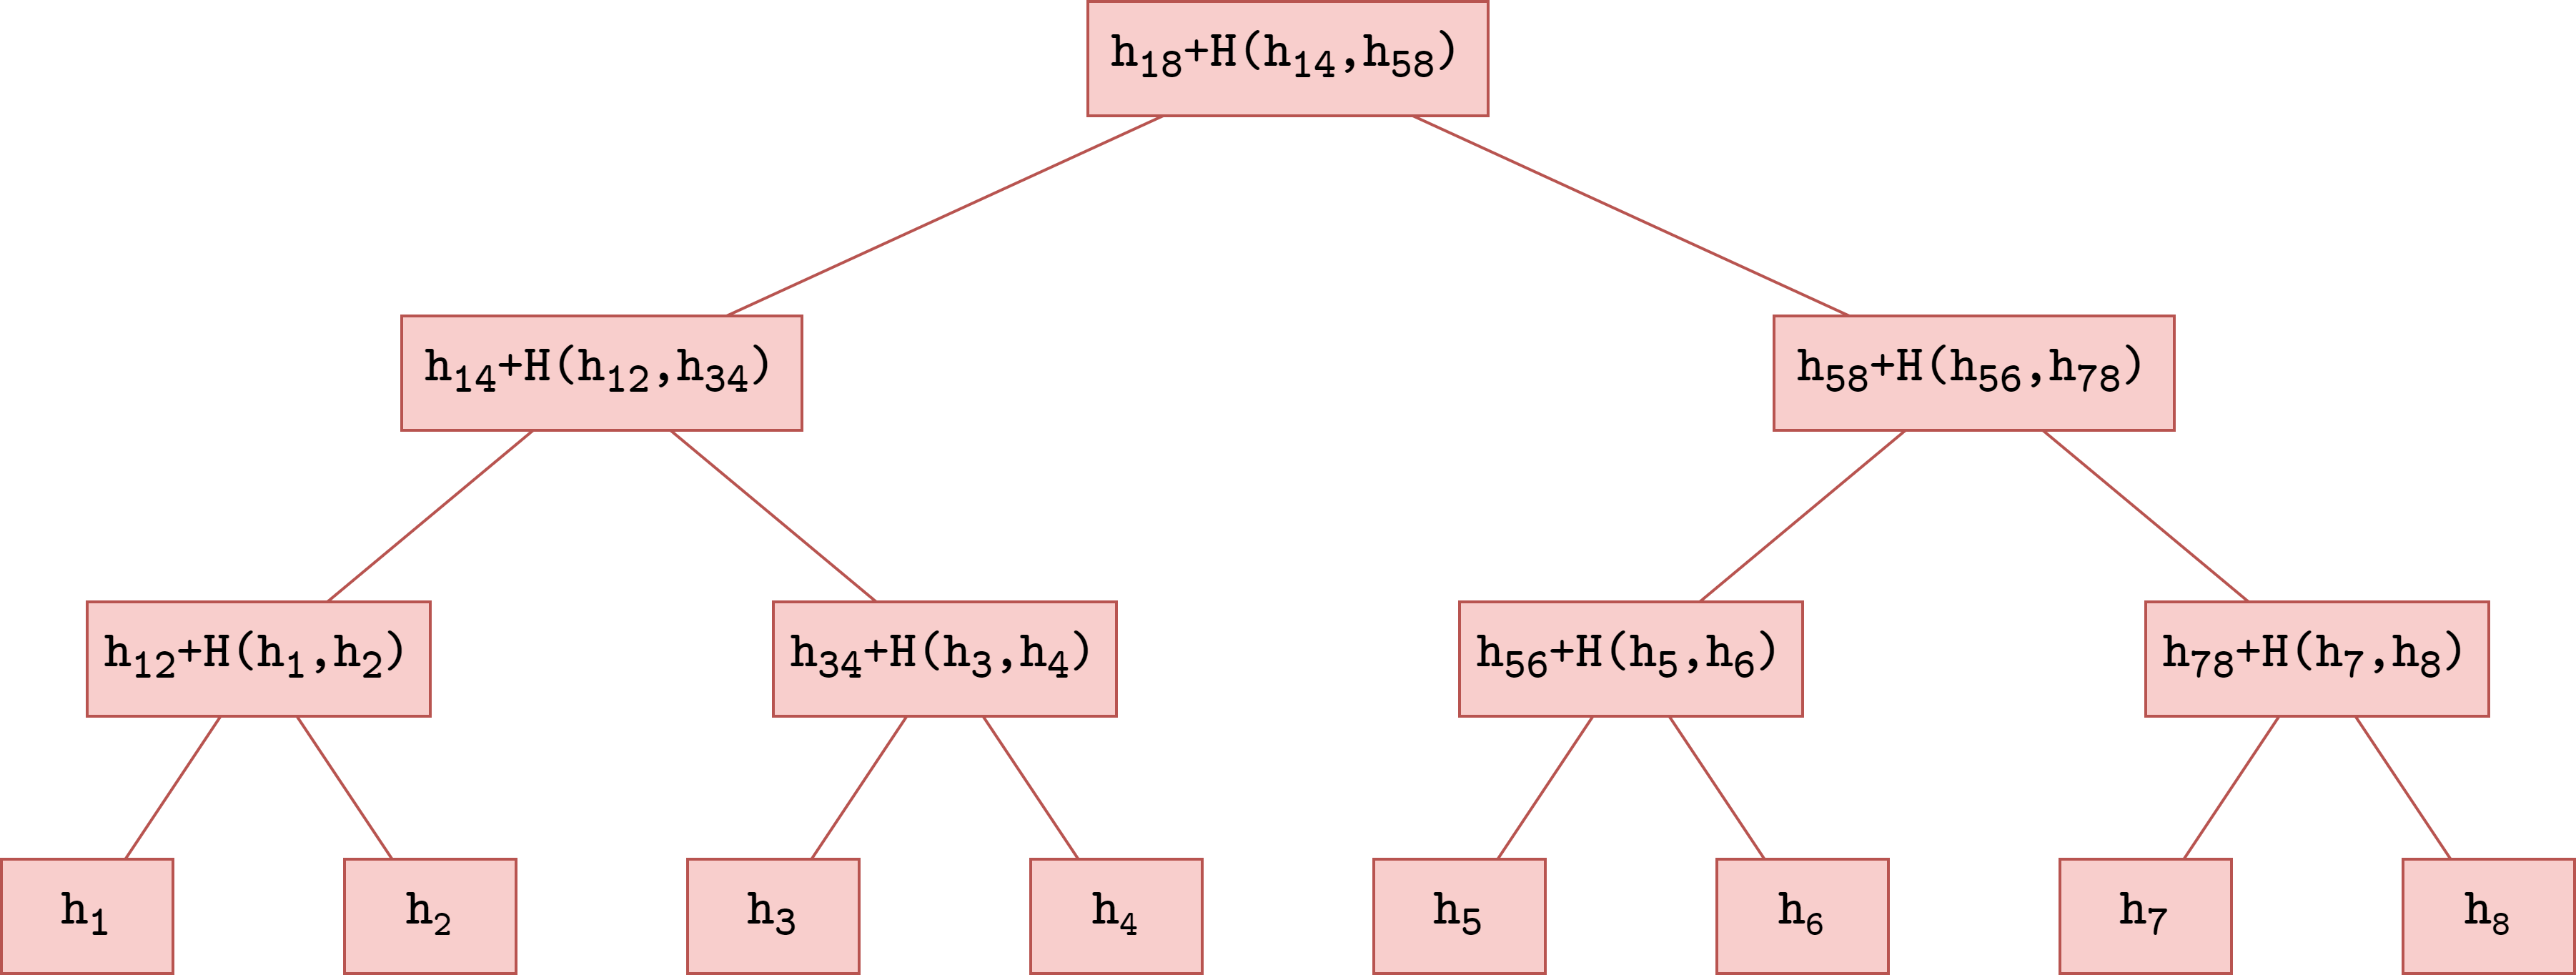
\includegraphics[width=10cm]{./Images/cap1/1.1.png}
\end{figure}

In questo modo posso calcolare gli hash due a due in modo da avere un solo hash alla fine, risparmiando tempo. Inoltre se ad esempio il proprietario del documento h\textsubscript{3} ha bisogno di controllare l'hash a partire da h\textsubscript{18}, ha bisogno solo degli hash di h\textsubscript{4}, h\textsubscript{12} e h\textsubscript{58}, quindi riduco il problema da lineare sul numero dei nodi a lineare sull'altezza. Se poi l'albero è bilanciato allora avrò risolto il problema utilizzando un numero di hash logaritmico sul numero dei nodi.

\subsection{MAC (Message Authentication Code)}
È una primitiva crittografica che prende in input un messaggio e una chiave segreta e genera un messaggio di autenticazione. Serve come applicazione sia per definire l'autenticità del messaggio sia per garantire la sua integrità (non serve invece per il non ripudio), in quanto se cambia il messaggio cambia anche il MAC.

Il MAC è diverso da una firma digitale perché non utilizza la chiave pubblica dell'utente ma la chiave privata, inoltre non c'è bisogno di un certificato perché è l'utente a generarlo automaticamente.

\subsection{Generatori pseudocasuali}
Nell'ambito della sicurezza, casuale vuol dire che per l'avversario che vuole attaccarci, le chiavi hanno tutte la stessa possibilità di essere scelte. Per scegliere valori casuali potrei utilizzare fattori impredicibili come la velocità del disco rigido in un determinato momento o la quantità di RAM utilizzata. Non conviene utilizzare il tempo in quanto se l'avversario sa che sto utilizzando il tempo può predire le mie mosse.

Tuttavia è molto oneroso generare bit casuali, per cui si utilizza la generazione pseudocasuale, usando algoritmi che prendono in input un seme di lunghezza fissata piccola, e forniscono una stringa di bit arbitrariamente grande. Un generatore pseudocasuale\footnote{Viene chiamato pseudocasuale perché l'algoritmo di generazione è deterministico, e non probabilistico.} è deterministico, quindi con semi uguali fornirà valori uguali. Il seme è l'unica variabile veramente casuale.

La sicurezza di un generatore pseudocasuale è data dalla sua indistinguibilità da un generatore casuale.

\subsection{Altre primitive crittografiche}
Come altre primitive non possiamo non menzionare l'autenticazione a due fattori, basata sulla combinazione di più primitive. In particolare l'autenticazione si deve basare su due delle seguenti caratteristiche:
\begin{itemize}
    \item qualcosa che l'utente possiede (carte fisiche o elettroniche, telefono)
    \item qualcosa che l'utente conosce (PIN, password);
    \item qualcosa che l'utente è (biometrie, impronte digitali).
\end{itemize}
Per quanto riguarda la sicurezza sul web il principale strumento di sicurezza è dato dal trasferimento dei dati tramite il protocollo HTTPS, molto diffuso negli ultimi anni grazie al fatto che è stato adottato dai motori di ricerca e dai social in tempi non sospetti. Per crittografare messaggi sul web si utilizzano anche tecniche di steganografia, magari mascherando i messaggi nei bit che determinano il colore di un pixel di un'immagine.

\vspace{5mm}

Altro strumento è dato dalla crittografia tramite curve ellittiche: in breve vengono utilizzate quando ci sono chiavi molto grandi, perché i numeri non sono indicati aritmeticamente ma come punti di curve ellittiche. In questo modo offrono lo stesso livello di sicurezza ma con minori lunghezze.

% \usepackage{colortbl}


\begin{table}
\centering
\begin{tabular}{|c|c|c|} 
\hline
\rowcolor[rgb]{0.753,0.753,0.753} \begin{tabular}[c]{@{}>{\cellcolor[rgb]{0.753,0.753,0.753}}c@{}}Cifrario\\simmetrico\\(grandezza chiave in bit)\end{tabular} & \begin{tabular}[c]{@{}>{\cellcolor[rgb]{0.753,0.753,0.753}}c@{}}\\Schema\\basato su ECC\\(grandezza di n in bit)\\\end{tabular} & \begin{tabular}[c]{@{}>{\cellcolor[rgb]{0.753,0.753,0.753}}c@{}}RSA/DSA\\(grandezza modulo in bit)\end{tabular}  \\ 
\hline
56                                                                                                                                                             & 112                                                                                                                             & 512                                                                                                              \\ 
\hline
80                                                                                                                                                             & 160                                                                                                                             & 1024                                                                                                             \\ 
\hline
112                                                                                                                                                            & 224                                                                                                                             & 2048                                                                                                             \\ 
\hline
128                                                                                                                                                            & 256                                                                                                                             & 3072                                                                                                             \\ 
\hline
192                                                                                                                                                            & 384                                                                                                                             & 7680                                                                                                             \\ 
\hline
256                                                                                                                                                            & 512                                                                                                                             & 15360                                                                                                            \\
\hline
\end{tabular}
\end{table}

\section{Cifrari a blocchi}
\subsection{Data Encryption Standard (DES)}
Il DES fu sviluppato a seguito delle richieste per uno standard nel 1973 e nel 1974 da parte della NBS (National Bureau of Standards), oggi NIST. La risposta si ebbe nel 1975 quando IBM presenta DES: il quale era una versione modificata di Lucifer, l'algoritmo di cifratura proprietario di IBM, la cui chiave era stata modificata passando da 128 bit a 56 bit per migliorare le prestazioni (La complessità dell'algoritmo dipende esponenzialmente sulla lunghezza delle chiavi). DES fu pubblicato ufficialmente il 15 gennaio 1977 (FIPS PUB 46) e doveva essere riaffermato ogni 5 anni. Fu infatti riaffermato nel 1983, nel 1987, nel 1992 e nel 1999 (quest'ultimo nonostante le DES challenges, sfide in cui si offriva un premio in dollari a chi riusciva a bucare l'algoritmo). Il 26 novembre 2001 fu pubblicato AES (Advanced Encryption Standard), e DES fu ritirato nel 2005. Attualmente DES può essere ancora utilizzato con la sua versione di triplo DES, il quale offre una quantità di sicurezza per utilizzi che non richiedono sicurezza troppo elevata. 

DES prende in input stringhe di 64 bit e produce in output stringhe di 64 bit. La chiave effettiva è di 56 bit anche se la lunghezza della chiave è di 64 bit, in quanto è presente un bit di parità ogni 7 bit (è lo XOR dei precedenti bit). Il DES è un cifrario di Feistel in quanto è a blocchi e prevede che si verifichino delle iterazioni per calcolare la schedulazione della chiave: vengono generate 16 sottochiavi, ognuna di lunghezza 48 bit, che va in input all'iterazione. Rispetto ad un cifrario semplice di Feistel il DES ha due blocchi in più, uno che esegue una permutazione fissa della chiave all'inizio e uno che esegue l'inverso della permutazione prima di restituire il testo in chiaro. La permutazione non dipende dalla chiave, e non rende l'algoritmo di molto più sicuro: è solo un modo per utilizzare anche i bit di parità.

\begin{figure}[htb!]
    \centering
    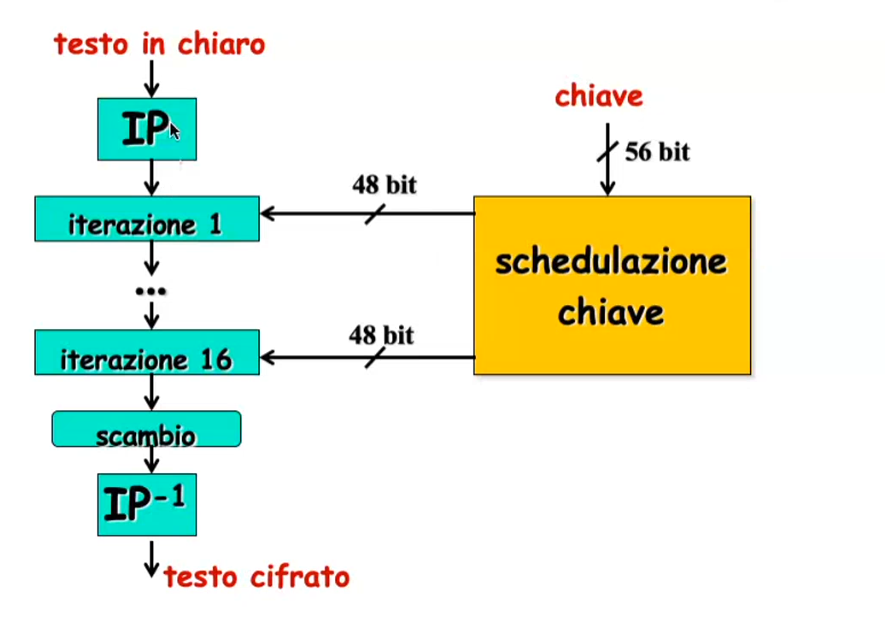
\includegraphics[width=6cm]{./Images/cap1/1.2.png}
\end{figure}

Il DES funziona come un cifrario di Feistel, per cui la struttura interna è pressoché la stessa:

\begin{figure}[htb!]
    \centering
    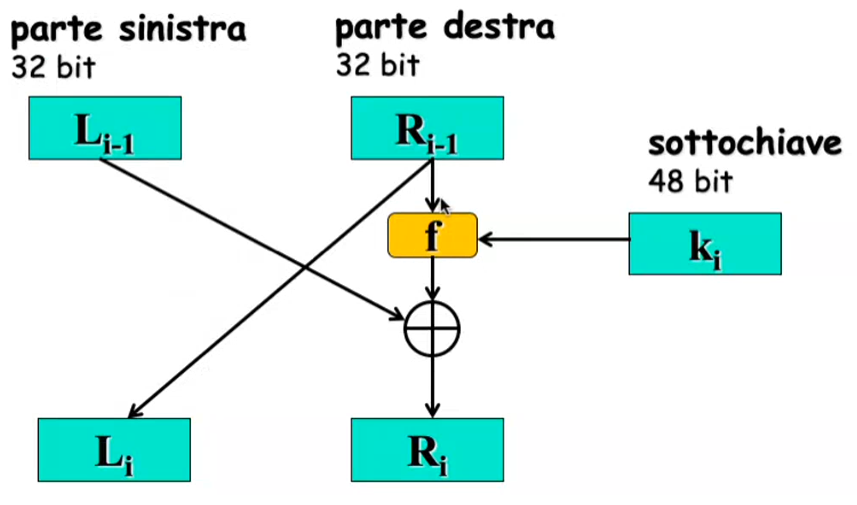
\includegraphics[width=6cm]{./Images/cap1/1.3.png}
\end{figure}

Visto che la lunghezza dell'iterazione è 64 bit, la parte sinistra e la parte destra sono di 32 bit ciascuna, con la sottochiave di 48 bit. Ci resta da definire la funzione f, in quanto l'unica non fissata.

La funzione f prende come input la parte destra di 32 bit e la sottochiave di 48 bit. Viene quindi fatta un'espansione di 16 bit (anche questa fissata) in cui la metà dei bit viene duplicata per permettere lo XOR successivo con la sottochiave. Dopodiché la stringa viene divisa in 8 parti da 6 bit ciascuna e data in input a 8 substitution box (o s-box) che restituiscono una stringa da 4 bit ognuna. La stringa finale da 32 bit viene permutata e poi restituita in output.

\begin{figure}[htb!]
    \centering
    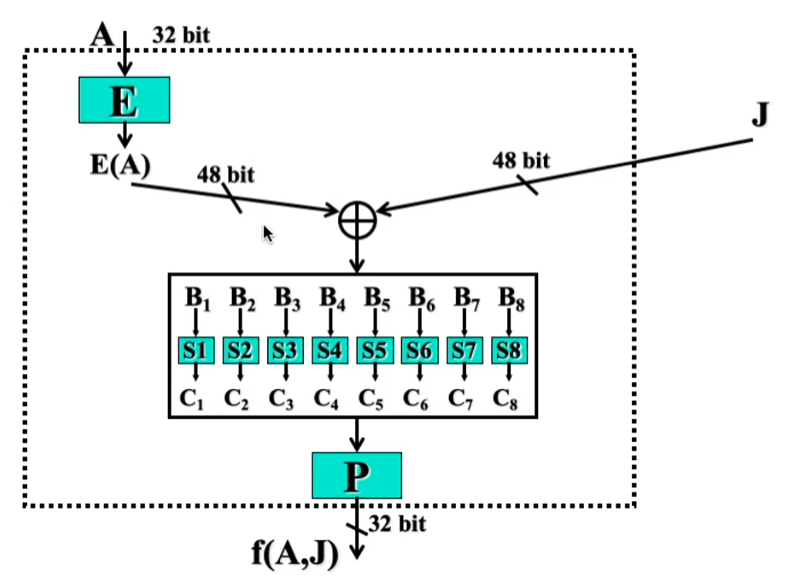
\includegraphics[width=6cm]{./Images/cap1/1.4.png}
\end{figure}

Il funzionamento di una s-box è molto semplice: i 6 bit ricevuti in input vengono interpretati in questo modo:
\begin{itemize}
    \item i 4 bit centrali diventano indici di colonna
    \item il bit iniziale e quello finale diventano indici di riga
\end{itemize}

\begin{figure}[htb!]
    \centering
    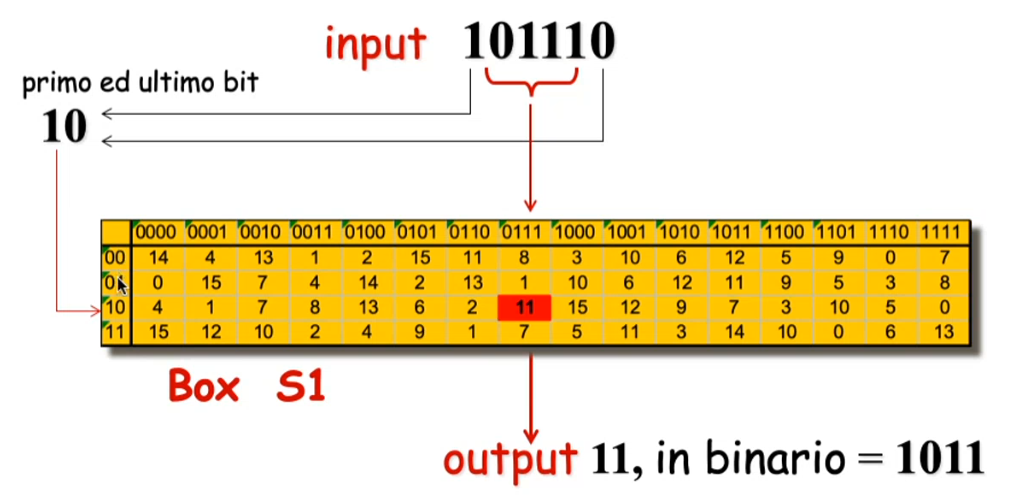
\includegraphics[width=8cm]{./Images/cap1/1.5.png}
\end{figure}

Proprietà delle s-box:
\begin{itemize}
    \item Le s-box non esprimono funzioni lineari
    \item Ogni riga è una permutazione degli interni 0, ..., 15
    \item Cambiando un solo bit di input ad una s-box cambiano almeno due bit nell'output
    \item Per ogni s-box S e per ogni input x a 6 bit vale che S(x) e S(x $\oplus$ 001100) differiscono in almeno due bit
    \item Pe ogni s-box, per ogni input x e per ogni bit dg, vale che S(x) $neq$ (x $\oplus$ 11dg00)
    \item Per ogni s-box il numero degli input per quali il bit di output è 0 è circa uguale al numero degli input per i quali tale bit è 1.
\end{itemize}
Nel passaggio da 56 bit a 48 bit vengono soppressi 8 bit. Essendo un cifrario di Feistel, la decifratura avviene in modo simile ma in senso opposto, ovvero con lo stesso algoritmo la con le sottochiavi in ordine inverso. L'algoritmo DES, come la maggior parte dei cifrari a blocchi, presenta un Avalanche Effect, ovvero un piccolo cambiamento del testo in chiaro oppure della chiave produce un grande cambiamento del testo cifrato.

Per provare un attacco brute force a un cifrario DES sono necessarie 2\textsuperscript{56} operazioni, difficili negli anni 70 ma fattibili al giorno d'oggi. Nel 1997, durante una delle DES challenges, fu eseguito un attacco di forza bruta e dopo 96 giorni gia erano state controllate il 24\% delle chiavi.

\vspace{5mm}

Sul DES esistono anche attacchi più sofisticati che attaccano in base alla struttura del DES e non sulla chiave: in particolare abbiamo la crittoanalisi differenziale (Biham e Shamir, 1990) e la crittoanalisi lineare (Matsui, 1993).
La crittoanalisi differenziale analizza come le differenze in input diventano differenze in output. La differenza in genere è lo XOR nell'analisi dei differenziali per ogni s-box ($\Delta X, \Delta Y$, dove $\Delta Y = S(X \oplus \Delta X) \oplus S(X)$. È molto efficace con un numero basso di iterazioni. DES è resistente alla crittoanalisi differenziale, ma con piccole modifiche diventa vulnerabile. La crittoanalisi lineare invece e più efficiente e lavora diversamente: recupera la chiave a partire da 2\textsuperscript{47} coppie (plaintext, ciphertext) di testi noti.

Il DES può lavorare in diverse modalità operative (ECB, CBC, CFB, OFB). Il più semplice è l'\textbf{Electronic Codebook Chaining} (ECB) in cui il messaggio in chiaro viene diviso in blocchi di 64 bit e vengono cifrati indipendentemente utilizzando sempre la stessa chiave e poi vengono concatenati. Per decifrare basta fare l'inverso in quanto la chiave è sempre la stessa. È possibile utilizzare la parallelizzazione per svolgere più operazioni contemporaneamente perché non c'è un ordine preciso delle operazioni da svolgere. L'ECB è il metodo più veloce ed eventuali errori non si propagano, inoltre non c'è dipendenza tra i blocchi. Non è sicuro per messaggi lunghi, in quanto allo stesso blocco in chiaro corrisponde sempre lo stesso cifrato.

\begin{figure}[htb!]
    \centering
    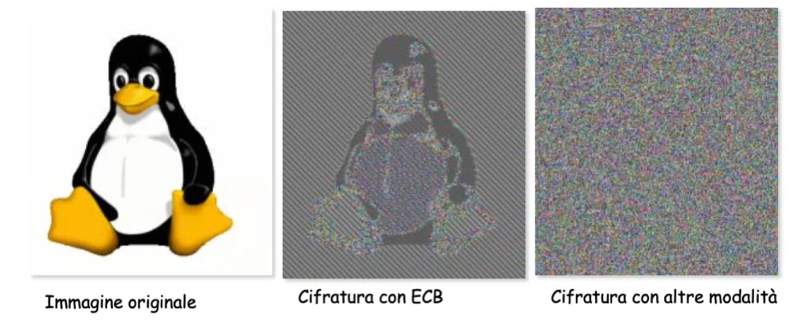
\includegraphics[width=9cm]{./Images/cap1/1.6.png}
\end{figure}

La modalità \textbf{Cipher Block Chaining} (CBC) divide il messaggio in chiaro in blocchi di 64 bit utilizzando un vettore di inizializzazione IV, di solito pubblico. La cifratura avviene applicando lo XOR e poi il DES, per decifrare si applica prima il DES\textsuperscript{-1} e poi lo XOR. Non è possibile parallelizzare la cifratura perché ogni valore dipende da quello precedente. È possibile invece parallelizzare la decifratura perché per decifrare y\textsubscript{i} è necessario avere x\textsubscript{i} e y\textsubscript{i-1}, che ho già a disposizione, quindi è possibile.
Nel caso di decifratura con IV errato l'errore è confinato solo nei primi 64 bit, quindi il messaggio si inizia a contare dal 65 esimo bit. Questo metodo ad esempio viene utilizzato nel protocollo TLS 1.1. La modalità CBC è meno veloce dell'ECB e se c'è un errore questo si propaga per tutti i bit seguenti. I vantaggi però sono la dipendenza dai blocchi, quindi aumenta la sicurezza, e non permette attacchi di sostituzione.

\vspace{5mm}

La modalità Cipher Feedback (CFB) non fa lo XOR con il messaggio cifrato ma lo XOR si trova dopo il DES e non prima del DES. La cifratura non è parallelizzabile perché c'è bisogno sempre della cifratura del valore precedente, il processo è sequenziale. La decifratura invece è parallelizzabile perché non ho bisogno della decifratura del valore precedente ma basta il testo cifrato. Se proviamo a decifrare usando un IV errato, solo il primo blocco è errato, come nel caso precedente.

\begin{figure}[htb!]
    \centering
    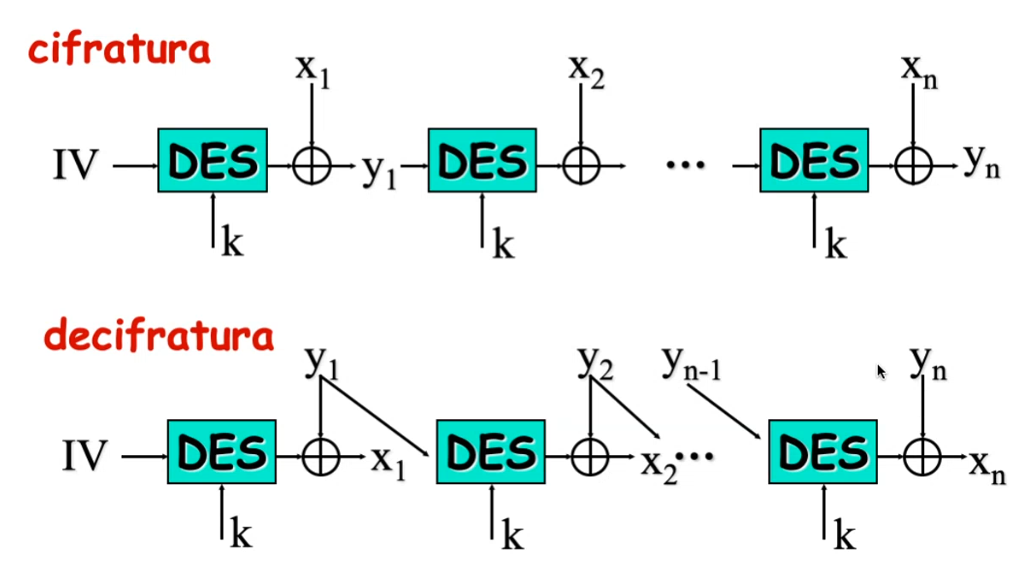
\includegraphics[width=7cm]{./Images/cap1/1.7.png}
\end{figure}  

Esiste una variazione di questo metodo chiamata j-bit, che consiste nel cifrare j bit alla volta invece che 64. Il valore j viene fissato a priori e concordato tra le parti.

\begin{figure}[htb!]
    \centering
    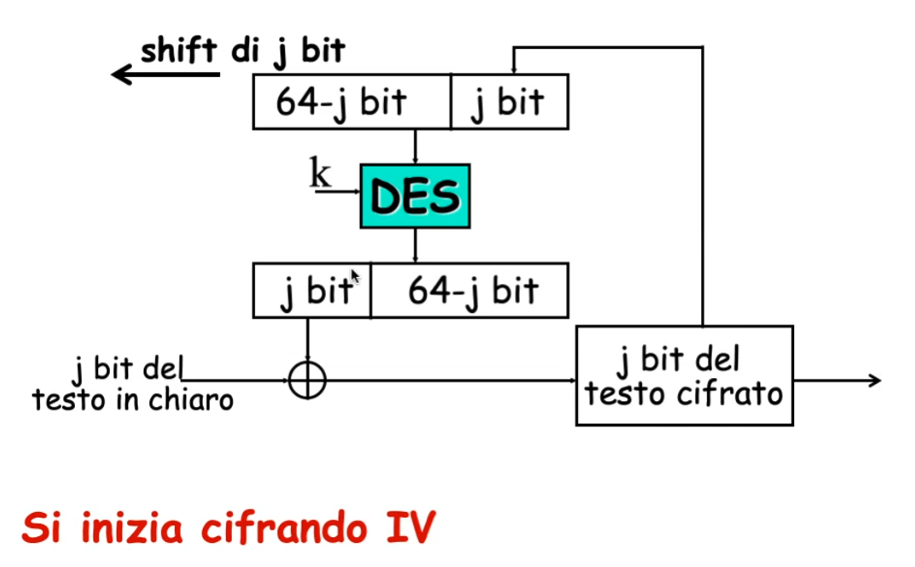
\includegraphics[width=6cm]{./Images/cap1/1.8.png}
\end{figure}

Il vantaggio della cifratura a j-bit sta che j può essere scelto a piacimento e si possono utilizzare j bit cifrati senza aspettarne 64. Lo svantaggio è che è lento al decrescere di j.

L'ultima modalità è l'Output Feedback (OFB), anch'essa supporta la versione a j-bit.

\begin{figure}[htb!]
    \centering
    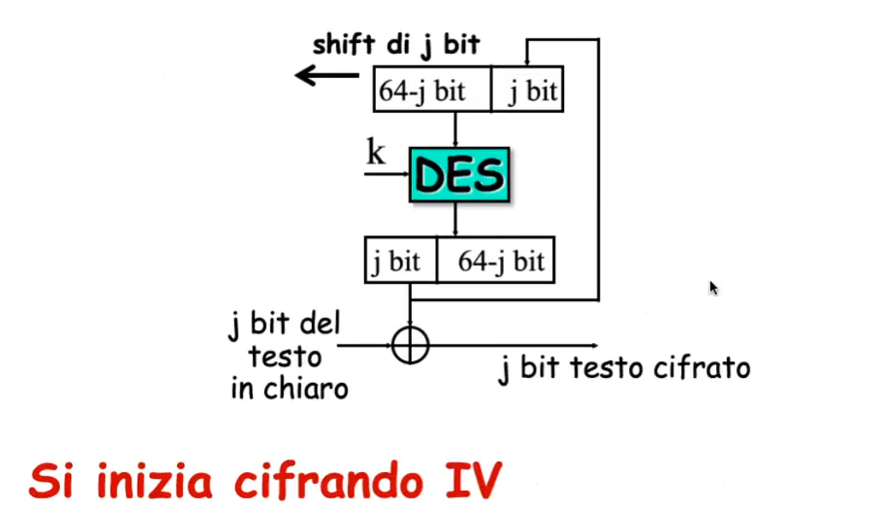
\includegraphics[width=6cm]{./Images/cap1/1.9.png}
\end{figure}

Il funzionamento è molto simile al precedente ma la differenza è che i j bit del testo in chiaro vanno in XOR con i j bit del testo cifrato che va in input al DES: infatti i valori input allo XOR possono essere precomputati. I vantaggi sono gli XOR facili da realizzare e non c'è dipendenza tra i blocchi. Tuttavia cambiando un bit nel testo in chiaro cambia un solo bit nel testo cifrato.

Un'altro metodo di cifratura che utilizza il DES è il Counter, che utilizza un contatore di 64 bit. Il messaggio viene diviso in blocchi di 64 bit e ogni blocco viene cifrato fissando un valore del contatore e facendo lo XOR tra il testo in chiaro e il valore ottendo il testo cifrato. Per il blocco successivo si aumenta il contatore di 1 e si fa lo XOR tra il valore del contatore e il testo in chiaro. Utilizzando lo stesso contatore di un blocco già utilizzato si otterrebbero correlazioni tra i relativi blocchi di testo in chiaro. I vantaggi sono efficienza hardware e software, pre-elaborazione e accesso casuale.

\vspace{5mm}

Il \textbf{Ciphertext Stealing} è un metodo per evitare un'espansione del testo cifrato quando la sua lunghezza non è multipla del blocco del cifrario (di solito 64 bit). Questa situazione si pone nel caso in cui si si vuole che le informazioni cifrate abbiano la stessa lunghezza delle informazioni in chiaro. Vediamo il funzionamento supponendo di avere un algoritmo di cifratura che usa la modalità CBC:

\begin{figure}[htb!]
    \centering
    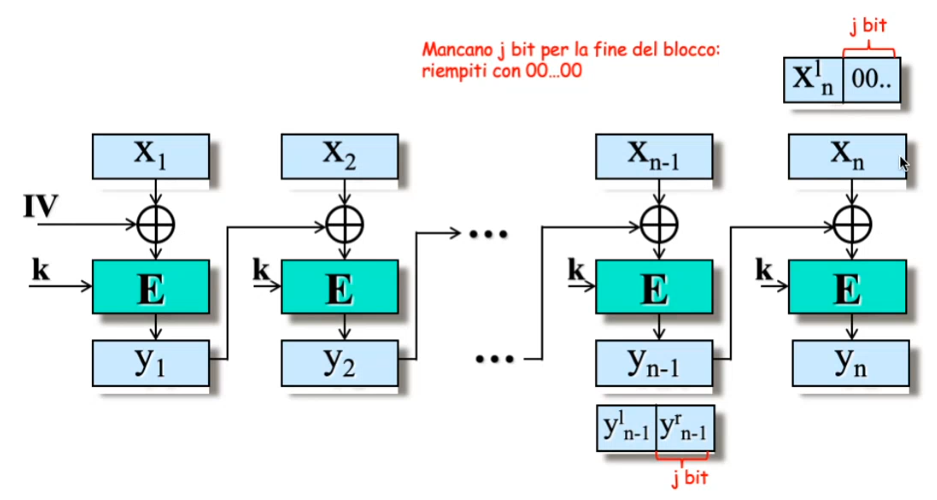
\includegraphics[width=6cm]{./Images/cap1/1.10.png}
\end{figure} 

Il penultimo valore y\textsubscript{n-1} non sarà trasmesso tutto ma saranno cancellati gli ultimi j bit. In questo modo viene tagliata una parte di messaggio ma la lunghezza è la stessa per cifrato e chiaro. Per decifrare si dovrà fare il processo inverso, ovvero si farà uno XOR tra j volte 0 e i bit che non sono stati messi nel messaggio cifrato: quando viene decifrato y\textsubscript{n}, gli ultimi suoi 8 bit sono proprio quelli che cercavo.

Le modalità viste finora implicano solamente la confidenzialità, mentre alcune come Counter CBC-MAC o Galois/Counter Mode utilizzano anche l'autenticazione. Infine ci sono anche cifrature che preservano il formato nel caso di dati non binari, e modalità che descrivono una protezione per le chiavi crittografiche.

\subsection{DES doppio e triplo}
L'idea della cifratura multipla nasce a causa della debolezza del DES, che ha una chiave piccola (56 bit). Per costruire un cifrario più sicuro a partire dal DES senza modificarne la struttura infatti si può usare ad esempio il DES doppio, che ha la lunghezza del blocco di 64 bit e la chiave lunga 56+56 = 112 bit. L'algoritmo di cifratura non fa altro che utilizzare il DES due volte, così come l'algoritmo di decifratura che decifra due volte partendo dalla fine.

\begin{figure}[htb!]
    \centering
    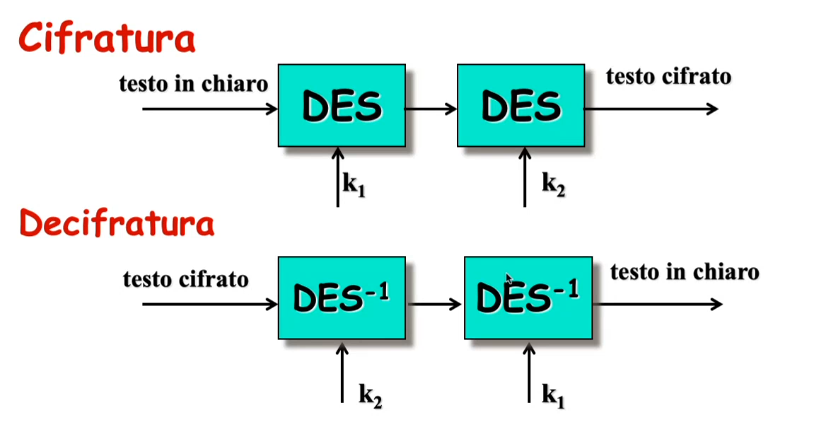
\includegraphics[width=7cm]{./Images/cap1/1.11.png}
\end{figure} 

La prima domanda che sorge è se esiste una chiave k\textsubscript{3} per ogni coppia di chiavi k\textsubscript{1}, k\textsubscript{2} tale che \textit{DES\textsubscript{k\textsubscript{3}}(c) = DES\textsubscript{k\textsubscript{2}}(DES\textsubscript{k\textsubscript{1}}(c))}. Ma ciò significherebbe che la cifratura singola è equivalente alla cifratura doppia. È stato dimostrato nel 1992 che esistono \textit{2\textsuperscript{64}!} \textit{>} \textit{10\textsuperscript{10\textsuperscript{20}}} permutazioni, corrispondenti ai \textit{{2\textsuperscript{64}}} input possibili. Ci sono invece \textit{{2\textsuperscript{56}}} << \textit{10\textsuperscript{10\textsuperscript{20}}} permutazioni definite dal DES: a ciascuna chiave DES fa corrispondere una permutazione. Se DES viene applicato due volte con chiavi diverse può produrre una delle permutazioni non definite da DES. Questo significa che l'insieme delle \textit{{2\textsuperscript{56}}} permutazioni definite dalle chiavi DES non è chiuso per composizione.

Esiste però un attacco al DES doppio che sotto particolari condizioni fa sì che la complessità computazionale necessaria per rompere il DES doppio non sia \textit{2\textsuperscript{112}} ma \textit{2\textsuperscript{56}}, e quindi rende inutile il DES doppio. L'attacco è di tipo Known Plaintext, per cui si conoscono coppie di messaggi (x,y) (con \textit{x} messaggio in chiaro e \textit{y} messaggio cifrato), ma non si conosce la chiave (k\textsubscript{1}, k\textsubscript{2}).

L'attacco si chiama \textit{meet in the middle} ed è molto semplice: data una coppia nota \textit{(x,y)}, basta cifrare \textit{x} con i \textit{2\textsuperscript{56}} valori possibili di k\textsubscript{1}, ottenendo così \textit{z}. A questo punto basta decifrare \textit{y} con i \textit{2\textsuperscript{56}} valori possibili di k\textsubscript{2}. Se trovo un match con \textit{z} allora ho trovato la chiave. In breve l'algoritmo potrebbe essere il seguente:

\begin{figure}[htb!]
    \centering
    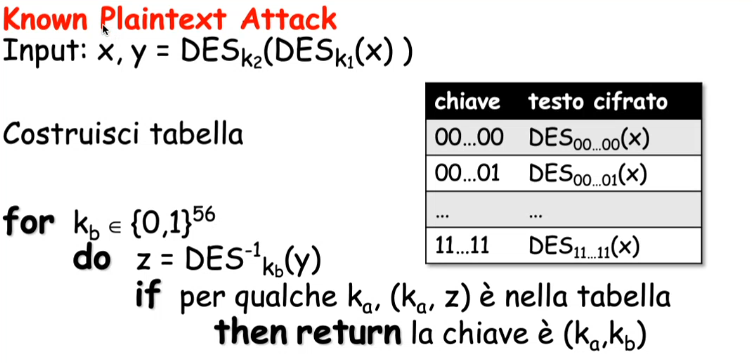
\includegraphics[width=6cm]{./Images/cap1/1.12.png}
\end{figure} 

La complessità di spazio è di 2\textsuperscript{56} (righe nella tabella), mentre la complessità di tempo è data dal prodotto di:
\begin{itemize}
    \item 2\textsuperscript{56} cifrature per x (costruzione tabella)
    \item 2\textsuperscript{56} per y
    \item 2\textsuperscript{56} ricerche in tabella:
        \begin{itemize}
            \item \textit{O(1)} se tabella hash
            \item 56 se array ordinato
        \end{itemize}
\end{itemize}
Quindi in totale è 2\textsuperscript{56}.

Si può calcolare il numero medio di chiavi per un valore cifrato tale che il DES doppio è equivalente al DES singolo. Vediamo come, facendo prima un esempio per un cifrario a blocchi con blocco di 2 bit e chiave di 3 bit: 

\begin{figure}[htb!]
    \centering
    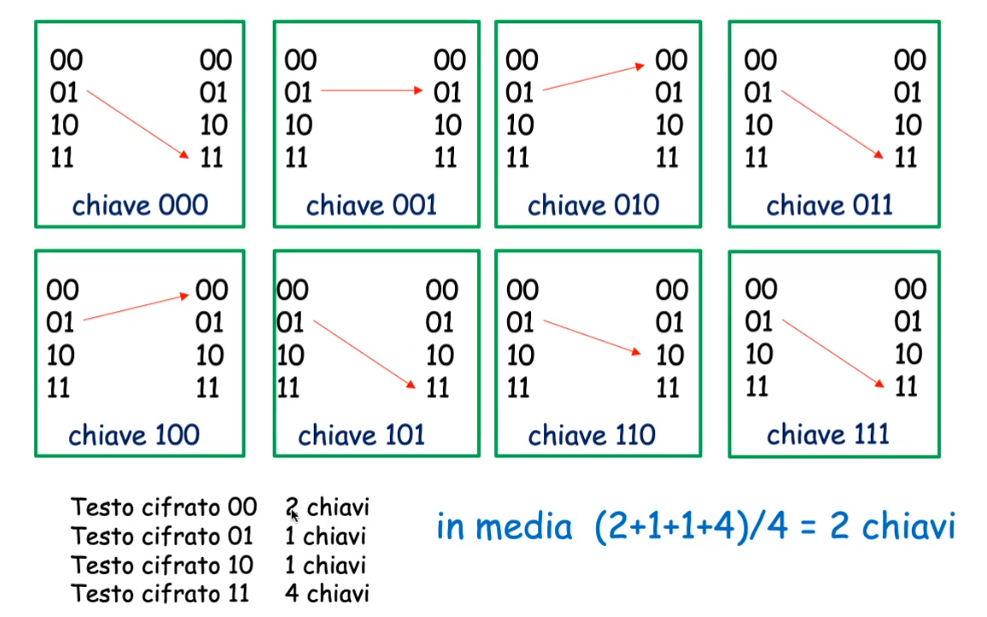
\includegraphics[width=8cm]{./Images/cap1/1.13.png}
\end{figure} 

Essendoci 8 possibili chiavi, il numero medio di chiavi è 2, fissando il valore iniziale. Tornando al DES doppio, fissato \textit{x}, abbiamo 2\textsuperscript{112} chiavi e 2\textsuperscript{64} testi cifrati y, per cui il numero medio di chiavi che cerchiamo è:

\begin{center}
    $\frac{2^{112}}{2^{64}} = 2^{48}$
\end{center}

Tuttavia è un numero di chiavi comunque elevato, per cui è possibile fare un'ulteriore modifica, ovvero utilizzare un'altra coppia (x,y) per verificare l'esattezza della chiave. Con questa modifica cambia il numero medio di chiavi ma costa di meno trovare la chiave perché nel momento che una chiave funziona per tutte e due le coppie allora è quella giusta con maggiore probabilità.

\begin{center}
    $\frac{2^{112}}{2^{128}} = 2^{-16}$
\end{center}

Per concludere, il DES doppio è vulnerabile ad un attacco di tipo \textit{meet in the middle}: la complessità (Known Plaintext) è circa \textit{2\textsuperscript{56}} mentre la ricerca esaustiva su tutte le chiavi è circa \textit{2\textsuperscript{112}}. Equivalente ad un cifrario con una chiave di 56 bit e non di 112 bit, e per questo non è mai stato utilizzato.

\vspace{5mm}


A questo punto si potrebbe pensare di aggiungere un ulteriore blocco alla cifratura utilizzando un DES triplicato.

\begin{figure}[htb!]
    \centering
    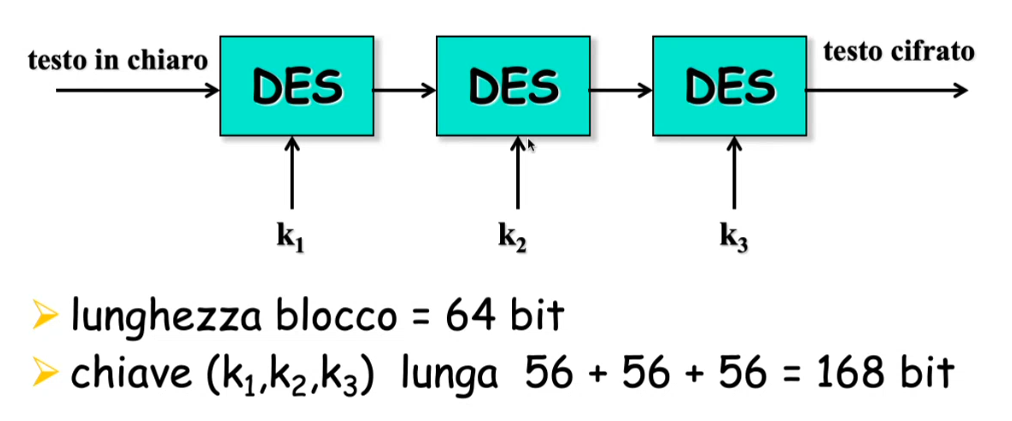
\includegraphics[width=6cm]{./Images/cap1/1.14.png}
\end{figure} 

Un attacco \textit{meet in the middle} può essere svolto anche su questo schema di cifratura, ponendosi ad esempio in mezzo tra il secondo e terzo blocco. Allo stesso modo precedente vediamo la costruzione dell'attacco:

\begin{figure}[htb!]
    \centering
    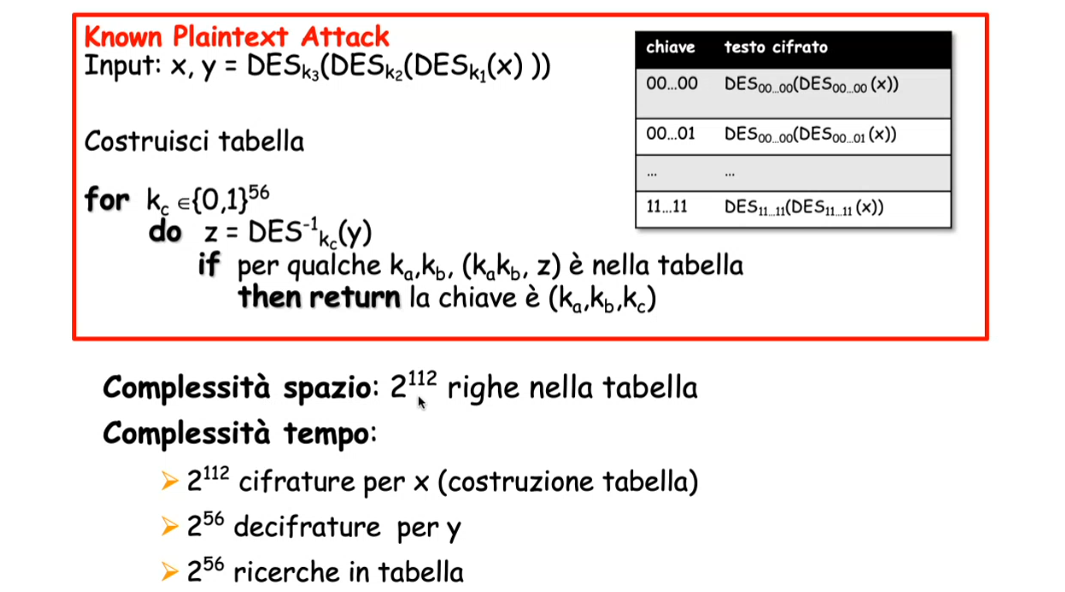
\includegraphics[width=6cm]{./Images/cap1/1.15.png}
\end{figure} 

Nonostante i numeri siano comunque elevatissimi, il metodo mostrato permette di far scendere la complessità dell'attacco da \textit{2\textsuperscript{168}} (ricerca esaustiva) a \textit{2\textsuperscript{112}}. Il DES triplicato diventa equivalente ad un cifrario a blocchi con chiave di 112 bit, e non 168.

Fatte queste considerazioni, si è pensato di utilizzare un DES triplo che utilizza solamente due chiavi:

\begin{figure}[htb!]
    \centering
    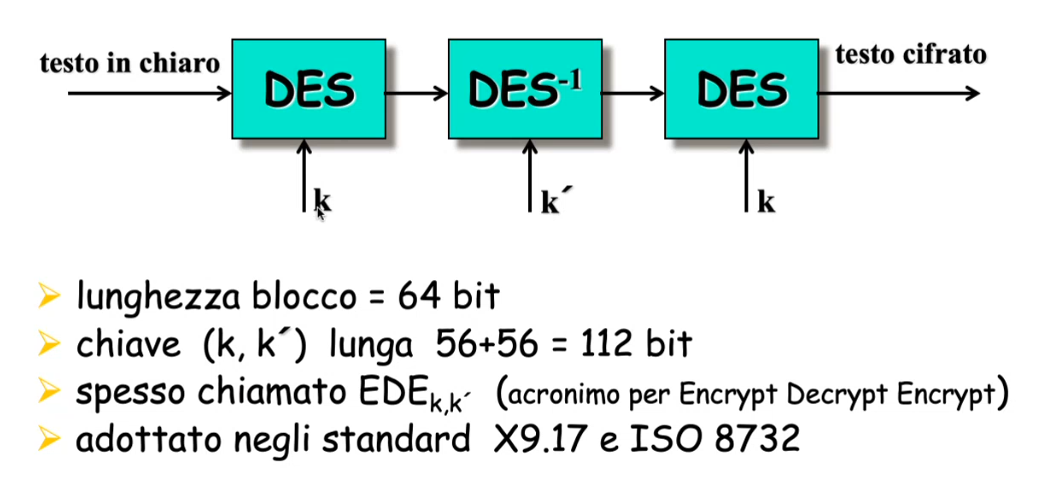
\includegraphics[width=6cm]{./Images/cap1/1.16.png}
\end{figure} 

Se provo ad effettuare un attacco \textit{meet in the middle} su questo cifrario la complessità è sempre \textit{2\textsuperscript{112}}. Non c'è però una debolezza in questo metodo di cifratura, perché la complessità è la stessa di un attacco di ricerca esaustiva sulle chiavi. Se le due chiavi sono uguali, il DES triplo coincide con il DES.

Il DES triplo viene chiamato anche TDEA (Triple Data Encryption Algorithm), con varianti come 2TDEA e 3TDEA (ovvero quello visto prima con tre chiavi differenti). Quest'ultima versione sarà valida fino al 2030 dopodichè dovrà essere sostituita con l'AES, che utilizza una chiave con lunghezza minima di 128 bit.

\subsection{Advanced Encryption Standard (AES)}

Un cifrario a blocchi più sicuro del DES è senza dubbio l'AES, reso effettivo dal NIST a partire da maggio 2002. I requisiti richiesti dal NIST erano:
\begin{itemize}
    \item Cifrario a blocchi
    \item Lunghezza della chiave variabile: 128, 192 o 256 bit
    \item Lunghezza del blocco di 128 bit
    \item Permette l'implementazione su smart card, le quali soffrono di prestazioni e memoria limitati.
    \item Royalty-free 
\end{itemize}

La selezione del NIST si è basata su sicurezza, efficienza di implementazioni hardware e software, e grandezza del codice e memoria utilizzata. Nell'immagine seguente è mostrata la struttura dell'AES.

\begin{figure}[htb!]
    \centering
    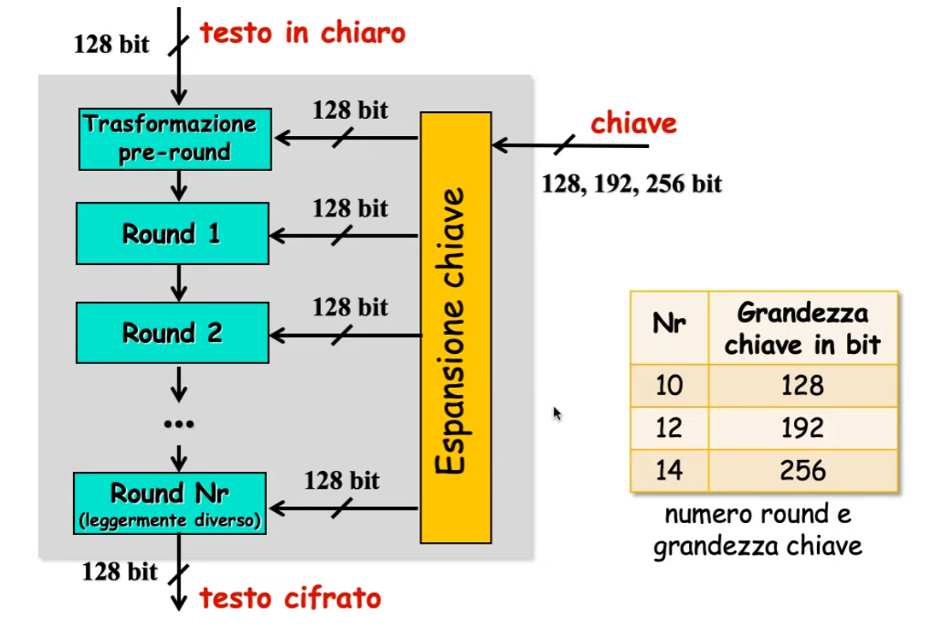
\includegraphics[width=8cm]{./Images/cap1/1.17.png}
\end{figure} 

Il funzionamento è simile a quello di altri cifrari a blocchi: ci sono una serie di round di cifratura che vengono effettuati uno dietro l'altro, che prendono in input l'output del messaggio precedente e 128 bit calcolati da un algoritmo di espansione della chiave. Il numero di round dipende dalla lunghezza della chiave (128, 192 o 256 bit).

L'AES non è un algoritmo di Feistel, quindi lavora sull'intero blocco in input e l'algoritmo di cifratura e quello di decifratura sono due algoritmi differenti. Usa operazioni facilmente ed efficentemente implementabili sia su architetture ad 8 bit (smartcard) sia a 32/64 bit. 

L'AES si basa sul concetto di stato, e tutti i dati sono salvati in una matrice di byte, che contiene 128 bit, detta appunto \textit{state}. Questa matrice è costituita da 4 righe e 4 colonne, le quali sono costituite da parole di 32 bit. Con \textit{S\textsubscript{r,c}} indichiamo il byte in riga \textit{r} e colonna \textit{c}. Le operazioni possono essere effettuate sia su parole di 8 bit (una cella) che su parole di 32 bit (una colonna). 

\begin{figure}[htb!]
    \centering
    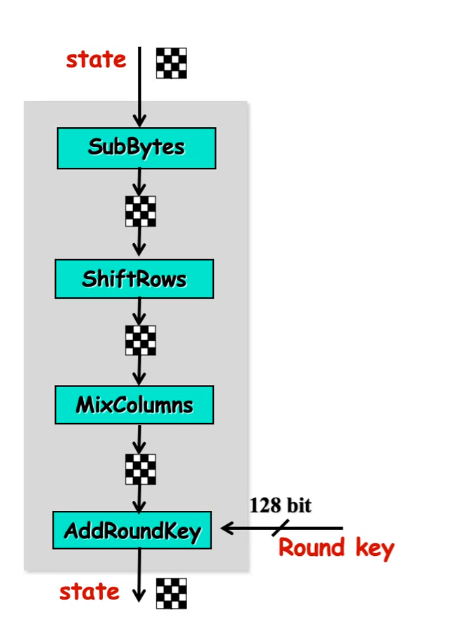
\includegraphics[width=6cm]{./Images/cap1/1.18.png}
\end{figure} 

Possiamo osservare la struttura di un round. Ogni round si compone di quattro operazioni, ognuna delle quali prende in input e restituisce il output i dati secondo la forma della matrice \textit{state}. Le operazioni sono SubBytes, ShiftRows, MixColumns e AddRoundKey.
\begin{itemize}
    \item \textbf{SubBytes} - ognuno dei 16 byte della matrice viene sostituito con un altro byte tramite una tabella di sostituzione (S-box);
    \item \textbf{ShiftRows} - ogni riga viene shiftata a sinistra in maniera ciclica di un certo numero di posizioni;
    \item \textbf{MixColumns} - vengono fatte operazioni matematiche per ogni colonna, la quale viene trattata come una parola di 32 bit. Le operazioni usano un'aritmetica sul campo finito GF(2\textsuperscript{8});
    \item \textbf{AddRoundKey} - l'ultima operazione consiste nello XOR bit a bit con la chiave di 128 bit espansa che viene passata in input.
\end{itemize}
Ogni round, come abbiamo visto, si ripete tante volte in base alla lunghezza della chiave. Prima del primo round c'è una trasformazione pre-round (AddRoundKeyMixColumns), mentre nell'ultimo round manca MixColumns. La copia dei dati iniziali (testo in chiaro) nella matrice di stato viene effettuata colonna per colonna da sinistra vestro destra. La stessa cosa viene effettuata per la copia finale dalla matrice di stato al testo cifrato. 

\begin{figure}[htb!]
    \centering
    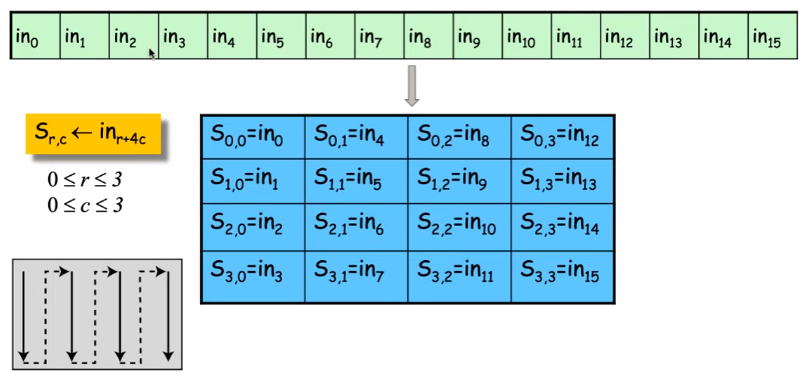
\includegraphics[width=8cm]{./Images/cap1/1.19.png}
\end{figure} 
  
Le operazioni matematiche effettuate su ogni byte avvengono in un campo finito, per cui il loro risultato sarà sempre un byte (8 bit, quindi 2\textsuperscript{8}=256 elementi). I valory dei byte sono rappresentati in notazione esadecimale, con due cifre esadecimali per ogni byte:

\[ 11010100 \rightarrow d4 \]

Ciascun byte è interpretato come un elemento del campo finito $GF(2^{8})$:

\[ 11010100 \rightarrow x^{7} + x^{6} + x^{4} + x^{2} \]

\textbf{Addizione in $GF(2^{8})$}: la somma corrisponde al polinomio i cui coefficienti sono la somma modulo due dei coefficienti dei due polinomi (in breve è lo XOR):

\[(x^{6} + x^{4} + x^{2} + x + 1) + (x^{7} + x + 1) = x^{7} + x^{6} + x^{4} + x^{2}\]
\[01010111 \oplus 10000011 = 11010100\]
\[57 \oplus 83 = d4\]

\textbf{Moltiplicazione in $GF(2^{8})$}: è definita in maniera tale che il risultato sia sempre un byte. Viene quindi effettuata una riduzione modulo $m(x)$, dove $m(x)$ è un polinomio, per cui viene fatta la divisione del risultato della moltiplicazione tra polinomi per $m(x)$, e il resto della divisione viene interpretato come risultato della moltiplicazione. Il polinomio $m(x)$ scelto per AES è $x^{8} + x^{4} + x^{3} + x + 1$, è di grado 8 ed è irriducibile, cosicché il resto della divisione entri in 1 byte. Le operazioni sono scelte in modo che siano associative e commutative, che abbiamo elemento neutro e inverso.

\begin{figure}[htb!]
    \centering
    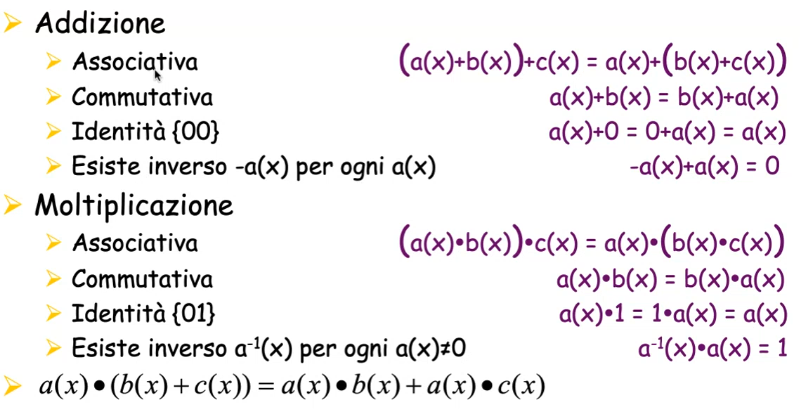
\includegraphics[width=8cm]{./Images/cap1/1.20.png}
\end{figure} 

Quindi la struttura è un campo finito su 256 elementi. Per rendere le operazioni efficienti computazionalmente ci sono due metodi: il primo consiste nel costruire una tabella 255x255 dove ogni entry è il byte che rappresenta il prodotto. la grandezza della tabella quindi è 65025 byte. C'è un metodo più efficiente che non richiede tabelle ma solo calcoli, e non effettua divisioni tra polinomi: consiste nello scompore uno dei due byte da moltiplicare in somma di byte che hanno un solo bit a 1, in questo modo le moltiplicazioni si riducono a shift a sinistra con un'eventuale somma di $m(x)$ visto prima\footnote{Un esercizio da fare potrebbe essere scrivere l'algoritmo per il calcolo delle moltiplicazioni}. 

\vspace{5mm}

La seconda parte dell'algoritmo riguarda le operazioni non piu su byte ma su parole di 32 bit. Si può estendere il concetto utilizzando un polinomi di grado 3 i cui coefficienti sono proprio i byte del primo passo.  
  
\begin{figure}[htb!]
    \centering
    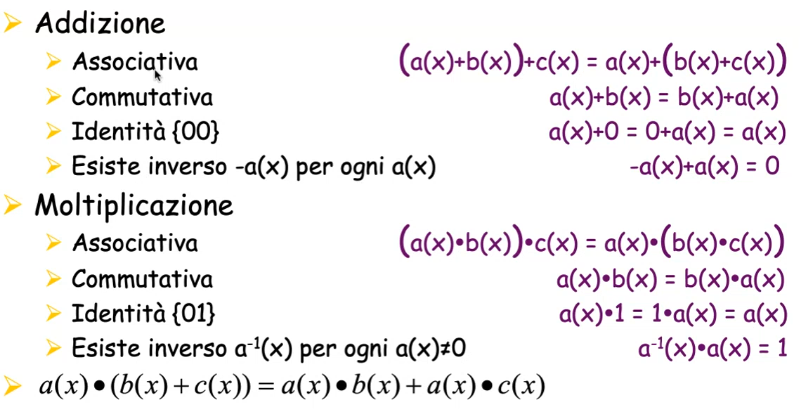
\includegraphics[width=9cm]{./Images/cap1/1.20.png}
\end{figure}   

Per implementare la somma tra i coefficienti delle parole di 32 bit mi basta fare lo XOR bit a bit tra i coefficienti, rendendo le operazioni molto efficienti. Per la somma tra le parole a 32 bit basta fare lo XOR tra le due intere stringhe binarie.

\begin{figure}[htb!]
    \centering
    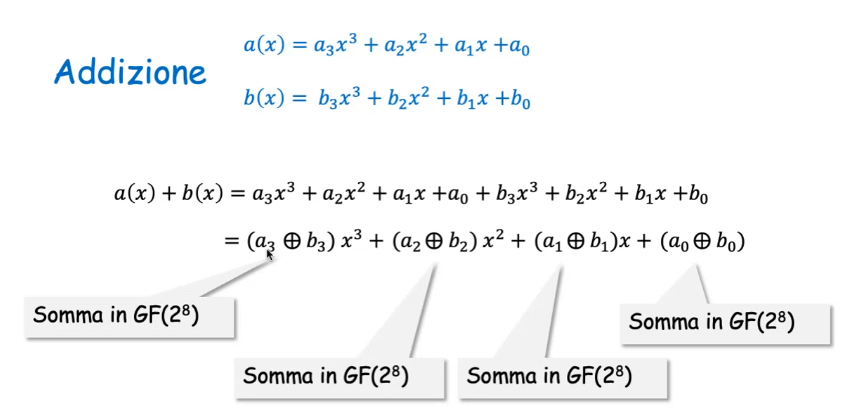
\includegraphics[width=8cm]{./Images/cap1/1.21.png}
\end{figure} 

Per la moltiplicazione si pone lo stesso problema precedente, ovvero il risultato non entra in una word, infatti il polinomio risultante ha grado 6, come si vede di seguito.

\begin{figure}[htb!]
    \centering
    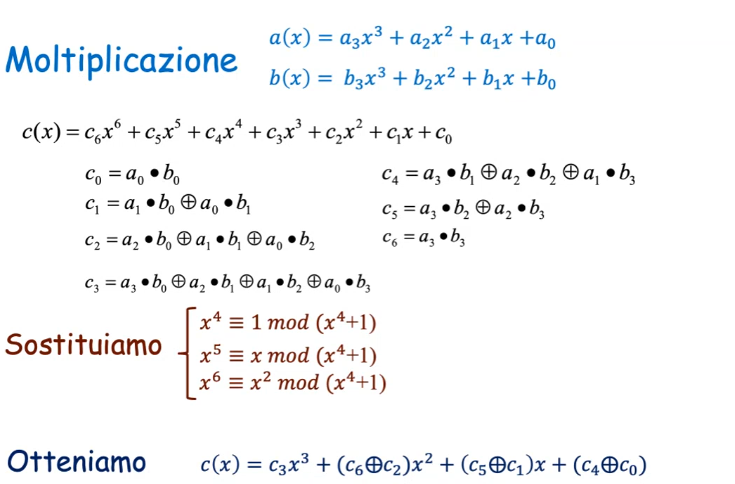
\includegraphics[width=8cm]{./Images/cap1/1.22.png}
\end{figure} 

Per ridurre il risultato della moltiplicazione per farlo entrare in una word di 32 bit si usa la riduzione modulo polinomio, che in questo caso è $x^{4} + 1$. Uso un polinomio di grado 4 perché il resto della divisione sarà di grado 3, quindi entrerà in 4 byte (32 bit). Si è scelto questo polinomio perché come si può vedere, quando si scelgono le potenze con grado maggiore e si applica l'operazione modulo, queste si riducono nell'esponente.

\begin{figure}[htb!]
    \centering
    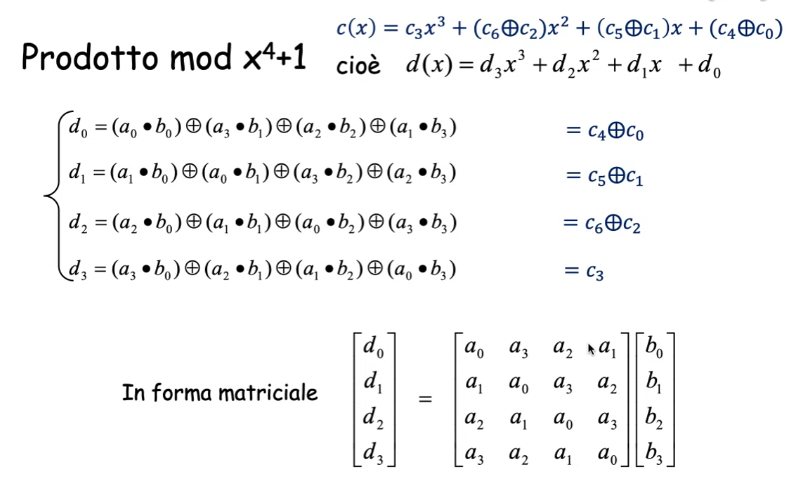
\includegraphics[width=10cm]{./Images/cap1/1.23.png}
\end{figure} 

Il polinomio $x^{4} + 1$ non è irriducibile su $GF(2^{8})$, e non tutti i polinomi hanno inverso $x^{4} + 1$. AES utilizza solamente questi polinomi:

\[a(x) = 03 x^{3} + 01 x^{2} + 01 x + 02\]
\[a^{-1}(x) = 0b x^{3} + 0d x^{2} + 09 x + 0e\]

Torniamo ora alle trasformazioni che vengono fatte in ogni round. La prima come abbiamo detto è SubBytes, illustrata nelle immagini seguenti:

\begin{figure}[htb!]
    \centering
    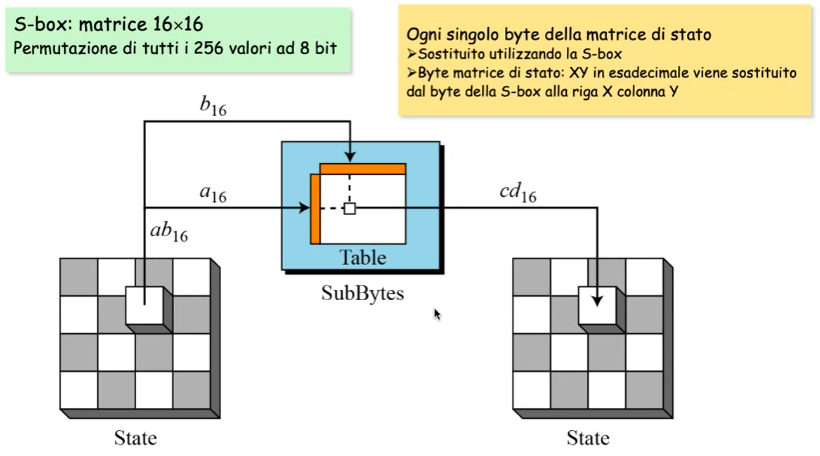
\includegraphics[width=9cm]{./Images/cap1/1.24.png}
\end{figure} 

\begin{figure}[htb!]
    \centering
    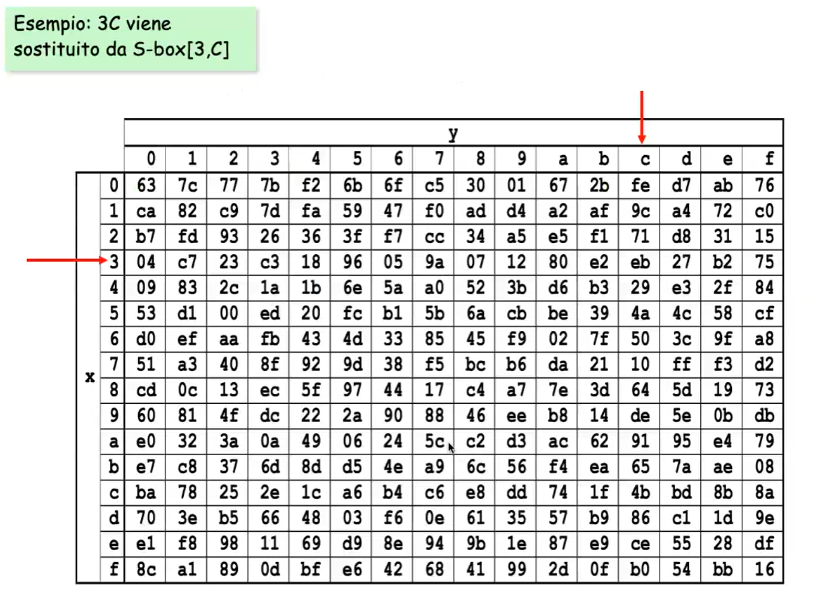
\includegraphics[width=0cm]{./Images/cap1/1.25.png}
\end{figure} 

La costruzione della S-box non è casuale ed è calcolata attraverso un insieme di operazioni:
\begin{enumerate}
    \item si inizializza la S-box con i valori dei byte in ordine ascendente riga per riga (00, 01, ..., 0F), (10, 11, ..., 1F), ...
    \item si sostituisce ciascun byte con il suo inverso moltiplicativo nel campo;
    \item si applica una trasformazione affine nel campo.
\end{enumerate}
La S-box AES soddisfa le seguenti proprietà:
\begin{itemize}
    \item l'output non è una funzione lineare dell'input;
    \item non ha punti fissi diretti né opposti (ovvero $S-box(a) \neq a$ e $S-box(a) \neq \overline{a}$);
    \item è invertibile (ovvero $Inverse_S-box(S-box(a)) = a$);
    \item non è self-invertibile ($Inverse_S-box(a) \neq S-box(a)$);
    \item è progettata per resistere ad attacchi crittoanalitici noti.
\end{itemize}

La trasformazione SubBytes ha quindi una sua inversa, detta InvSubBytes, che viene utilizzata nella decifratura. 

\vspace{5mm}

La seconda trasformazione (ShiftRows) è uno shift ciclico riga per riga: la prima riga non si muove, la seconda shifta a sinistra in maniera circolare di 1 byte, la terza di 2 byte e la quarta di 3 byte.

\begin{figure}[htb!]
    \centering
    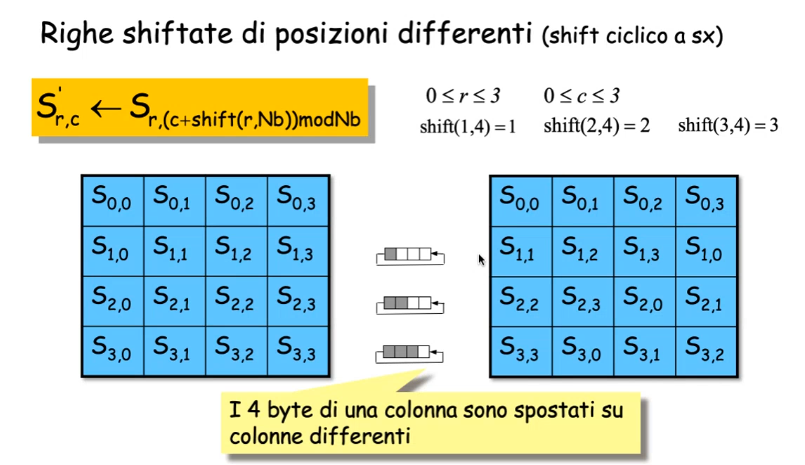
\includegraphics[width=9cm]{./Images/cap1/1.26.png}
\end{figure} 

La terza trasformazione (MixColumns) considera le 4 colonne e applica ad ognuna una moltiplicazione per il polinomio $a(x)$ (che ha un unico inverso) modulo il polinomio $x^{4} + 1$. Per la decifratura mi basterà moltiplicare le colonne per l'inverso di $a(x)$

\begin{figure}[htb!]
    \centering
    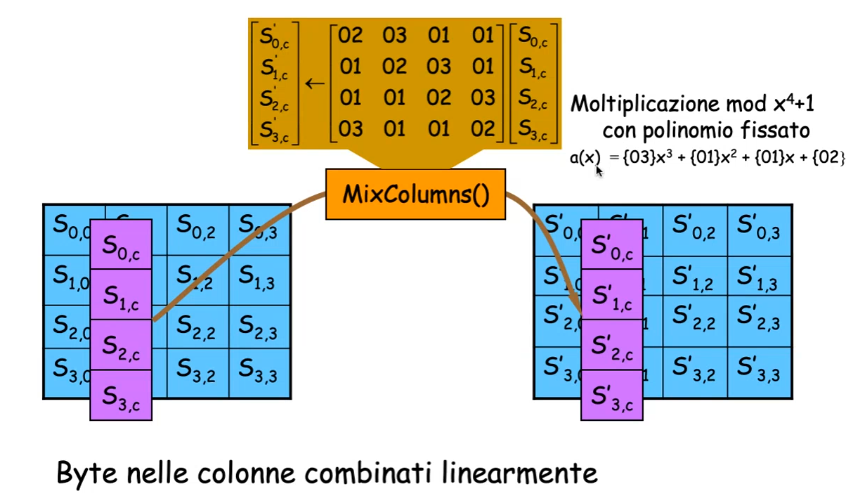
\includegraphics[width=9cm]{./Images/cap1/1.27.png}
\end{figure} 

L'ultima trasformazione non è altro che uno XOR bit a bit con l'espansione della chiave. L'algoritmo di espansione a partire dalla chiave (matrice \textit{key} di \textit{4*Nk} byte genera le chiavi schedulate (array \textit{w} di \textit{4*(Nr+1) word)}: 4 word per AddRoundKey iniziale e 4 word per AddRoundKey in ciascun round. Ad esempio, se Nk = 4 (chiave a 128 bit), sono prodotte 44 word (4 word per AddRoundKey iniziale e 4 word per ognuno dei 10 round.

L'algoritmo di decifratura non è lo stesso della cifratura, infatti usa una diversa sequenza di trasformazioni, e usa le inverse. Lo svantaggio ovviamente è che c'è bisogno di una doppia implementazione. Esiste la possibilità di utilizzare un algoritmo di decifratura che ha la stessa struttura di quello di cifratura, ma occorre effettuare un cambiamento nella schedulazione della chiave.

\begin{figure}[htb!]
    \centering
    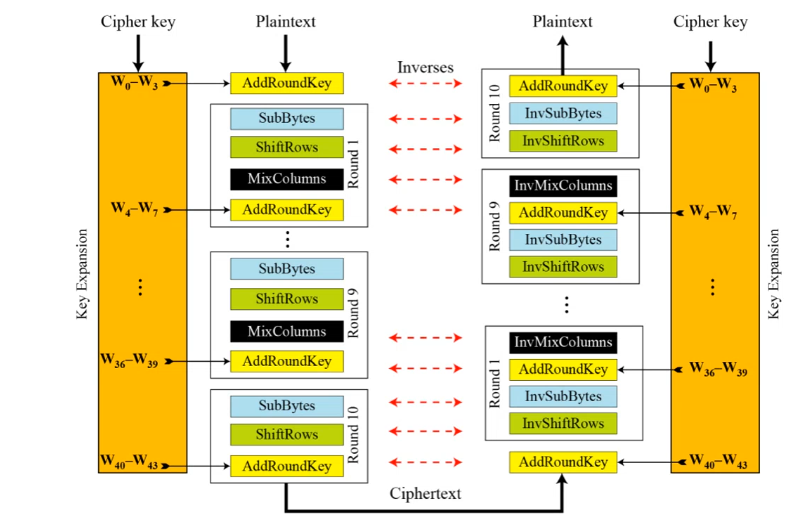
\includegraphics[width=10cm]{./Images/cap1/1.28.png}
\end{figure} 

Di seguito vediamo gli algoritmi di cifratura e di decifratura per l'AES:

\begin{lstlisting}[escapeinside={(*}{*)}]
Cipher (byte in[4*Nb], byte out[4*Nb], word w[Nb*(Nr + 1)])
    byte state[4,Nb]
    state (*$\leftarrow$*) in
    AddRoundKey (state, w)
    for round = 1 to Nr - 1
        SubBytes (state)
        ShiftRows (state)
        MixColumns (state)
        AddRoundKey (state, w + round * Nb)
    SubBytes (state)
    ShiftRows (state)
    AddRoundKey (state, w + Nr * Nb)
    out (*$\leftarrow$*) state
    
    
DeCipher(byte in[4*Nb], byte out[4*Nb], word w[Nb*(Nr+1)])
    byte state[4,Nb]
    state (*$\leftarrow$*) in
    AddRoundKey(state, w + Nr * Nb)
    for round = Nr - 1 step -1 to 1
        InvShiftRows(state)
        InvSubBytes(state)
        AddRoundKey(state, w + round * Nb)
        InvMixColumns(state)
    InvShiftRows(state)
    InvSubBytes(state)
    AddRoundKey(state, w)
    out (*$\leftarrow$*) state  
\end{lstlisting}

Anche l'AES è soggetto all'Avalanche effect: un piccolo cambiamento del testo in chiaro oppure della chiave produce un grande cambiamento del testo cifrato. 

Uno studio del NIST ha evidenziato come la standardizzazione dell'AES abbia portato ad un risparmio di circa 250 miliardi di dollari. Gli utilizzi dettati dalla legge sono mostrati di seguito.

\begin{figure}[htb!]
    \centering
    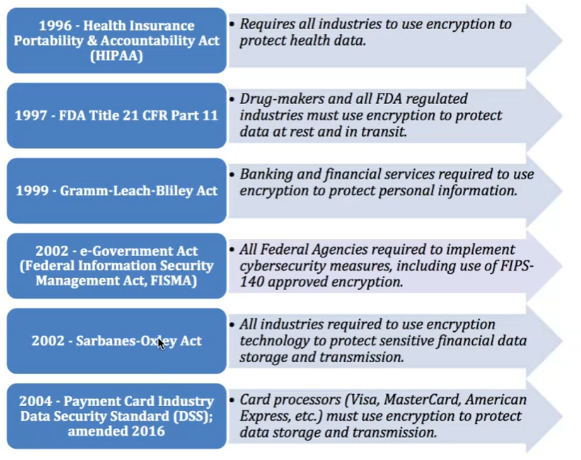
\includegraphics[width=9cm]{./Images/cap1/1.29.png}
\end{figure} 

\section{Stream Ciphers}
La differenza principale con i cifrari a blocchi è che i primi hanno bisogno di effettuare diverse operazioni in base alla lunghezza del messaggio da cifrare, perché questo va diviso in blocchi. I cifrari a flusso invece trasformano i singoli caratteri del testo in chiaro, e quindi risultano più efficienti dal punto di vista computazionale anche grazie alle semplici operazioni che devono compiere.

In genere uno stream cipher funziona in questo modo:
\begin{itemize}
    \item cifra il messaggio un byte (o bit) alla volta;
    \item utilizza una sequenza (\textbf{keystream}) pseudo-casuale generata a partire dalla chiave (e dal messaggio);
    \item cifra il messaggio mediante la keystream.
\end{itemize}

\begin{figure}[htb!]
    \centering
    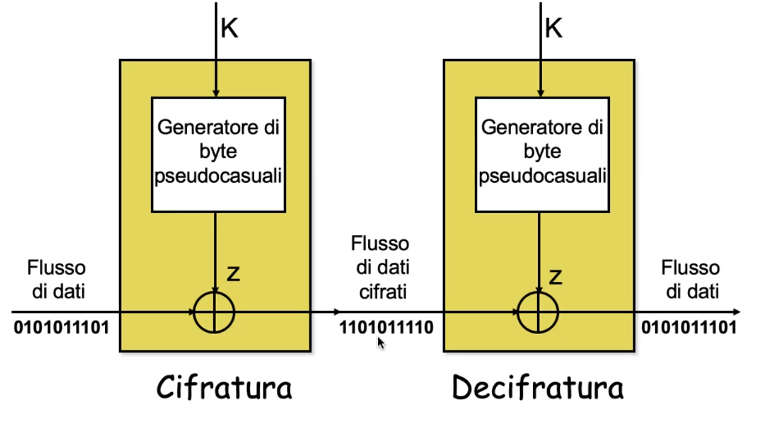
\includegraphics[width=8cm]{./Images/cap1/1.30.png}
\end{figure} 

Per complicare la crittoanalisi occorre utilizzare un keystream di lungo periodo: infatti il generatore pseudocasuale dopo un certo periodo inizia a ripetere gli stessi valori, e un attaccante potrebbe utilizzarlo per estrapolare le dipendenze statistiche nel testo. Si deve utilizzare inoltre un keystream con le stesse caratteristiche di una sequenza casuale, ad esempio dovrebbe avere all'incirca lo stesso numero di 0 e di 1, e allo stesso modo vista come sequenza di byte, ciascuno dei 256 valori dovrebbe apparire all'incirca lo stesso numero di volte.

\subsection{Linear Feedback Shift Register (LFSR)}
I registri del LFSR vengono definiti da una relazione di ricorrenza che lega il valore di indice \textit{i+m} agli \textit{m} valori precedenti:
\begin{center}
$z_{i + m} = c_{0}z_{i} + c_{1}z_{i+1} + ... + c_{m-1}z_{i+m-1}$ mod 2 $(i = 0,1,2,...)$
\end{center}



Ogni singolo bit in pratica è combinazione lineare dei bit precedenti: è una ricorrenza lineare di grado m. I valori $c_{0} ... c_{m-1}$ vengono fissati precedentemente. A partire dall'indice \textit{m} poi i valori successivi verranno definiti dalla ricorrenza che abbiamo appena visto. L'output del generatore è la sequenza composta da \textit{z}, che poi andrà in XOR con il testo in chiaro. Le proprietà in breve vengono definite da un polinomio di grado \textit{m-1} i cui coefficienti dei valori della \textit{x} sono le costanti di questa relazione di ricorrenza:

\[P(x) = c_{m-1}x^{m-1} + ... + c_{1}x  + c_{0}\]

La chiave è data dai valori di inizializzazione $k_{0} k_{1} ... k_{m-1}$ e dai coefficienti $c_{0} c_{1} ... c_{m-1}$. Non sempre però i coefficienti fanno parte della chiave, in quanto dipende dal tipo di implementazione, considerando anche che un eventuale attaccante può facilmente entrarne in possesso. Se la chiave è molto lunga questo evita la vulnerabilità ad attacchi basati sul periodo della chiave. L'implementazione dell'LFSR è molto efficiente e viene effettuata attraverso la costruzione di diversi registri a scorrimento. Vediamo un esempio per m = 4: abbiamo che \textit{c\textsubscript{0} = 1}, \textit{c\textsubscript{1} = 1}, \textit{c\textsubscript{2} = 0} e \textit{c\textsubscript{3} = 0}, da come si può vedere dai coefficienti della relazione esplicitata per \textit{z\textsubscript{i+4}}.

\begin{figure}[htb!]
    \centering
    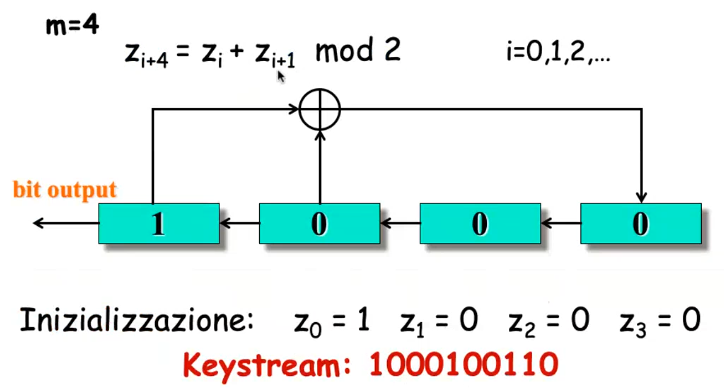
\includegraphics[width=8cm]{./Images/cap1/1.31.png}
\end{figure} 

Una volta fissata questa sequenza c'è bisogno dell'inizializzazione, quindi devo fissare 4 valori iniziali: \textit{z\textsubscript{0}}, \textit{z\textsubscript{1}}, \textit{z\textsubscript{2}} e \textit{z\textsubscript{3}}, rappresentati dai registri. A questo punto posso trovare tutti i valori successivi a partire da questi. Ad esempio, abbiamo che \textit{z\textsubscript{4}} = \textit{z\textsubscript{0}} + \textit{z\textsubscript{1}}, \textit{z\textsubscript{5}} = \textit{z\textsubscript{1}} + \textit{z\textsubscript{2}}, e così via. 

Vediamo ora l'implementazione hardware: i 4 registri ad ogni colpo di clock shiftano a sinistra e quello attualmente in posizione 0 va in output, ma i primi due vengono messi a XOR e vanno nell'ultimo registro, proprio come abbiamo definito la relazione. Appare quindi molto semplice da implementare a livello hardware.

\begin{figure}[htb!]
    \centering
    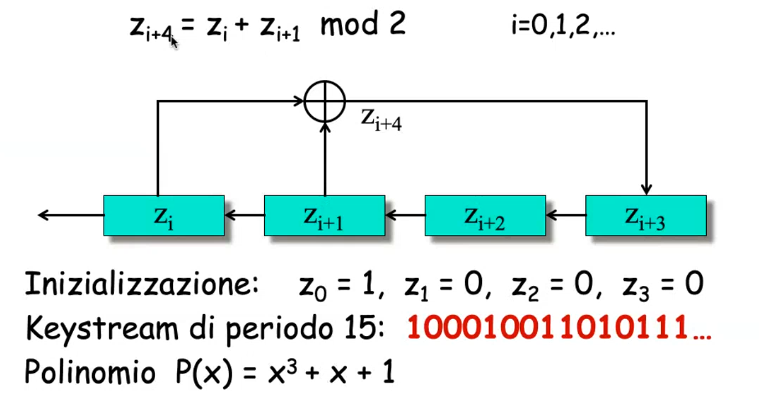
\includegraphics[width=8cm]{./Images/cap1/1.32.png}
\end{figure} 

Il periodo di questa specifica implementazione è 15: dopo 15 shift infatti i valori che saranno nei registri saranno gli stessi e quindi i valori in output si ripeteranno. In realtà avendo 4 registri, 15 è proprio il periodo massimo (\textit{2\textsuperscript{4} = 16}, ma la configurazione che non viene contata è quella con tutti zeri, altrimenti l'output sarebbe sempre 0). 

\subsubsection{\textbf{CRITTOANALISI}}
Supponiamo che non si conoscano i coefficienti $c_{0} c_{1} ... c_{m-1}$. Un possibile attacco è di tipo Known Plaintext, dove l'attaccante conosce il testo in chiaro $M_{0} M_{1} ... M_{n}$, il testo cifrato $Y_{0} Y_{1} ... Y_{n}$ e può calcolare $z_{0} z_{1} ... z_{n}$, infatti $z_{n} = M_{i} \oplus Y_{i}$.

Essendo l'LFSR un cifrario che utilizza solo relazioni lineari, l'attaccante potrebbe anche risalire alla chiave utilizzando appunto delle trasformazioni lineari, infatti si ha che:

\begin{figure}[htb!]
    \centering
    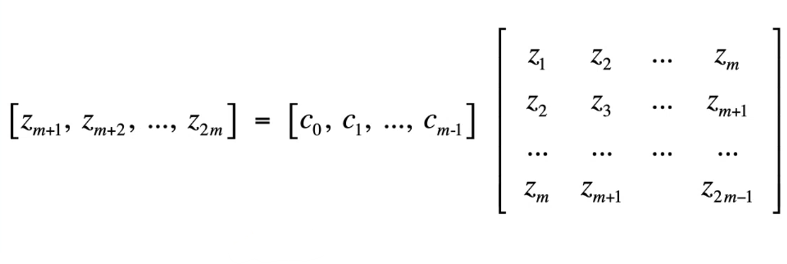
\includegraphics[width=10cm]{./Images/cap1/1.33.png}
\end{figure} 

Se la matrice ha determinante diverso da 0 è possibile moltiplicare i valori noti per l'inverso della matrice per trovare facilmente i valori cercati.

Il semplice registro a scorrimento non basta per garantire una sicurezza di base per cui quello che si fa è utilizzare diversi shift register in combinazione tra loro con una funzione non lineare che danno luogo a un vero e proprio stream cipher. Le proprietà desiderabili infatti sono proprio periodo lungo e non linearità delle funzioni utilizzate.

\subsection{A5 e GSM}
A5 è uno stream cipher utilizzato nel GSM (Group Spécial Mobile), standard di rete per le connessioni 2G. Fu sviluppato tra il 1987 e il 1989 prima in Europa e poi negli USA, e inizialmente l'algoritmo era segreto e fu scoperto solo nel 1999 da Marc Briceno con tecniche di reverse engineering. L'algoritmo si basa su tre LFSR di grado 19, 22 e 23 la cui chiave è memorizzata nella memoria della SIM (Subscriber Identity Module). Si noti che si parla sempre di crittografia simmetrica quindi con la stessa chiave privata, la quale è conosciuta dal gestore telefonico e viene immessa nella SIM dell'utente, quindi è come se le parti si "scambiassero" le chiavi. La chiave che si trova sulla SIM ha lunghezza di 64 o 128 bit. Il segnale viaggia cifrato solo dal dispositivo alla stazione base, mentre viene scambiato in chiaro tra le componenti di rete della stazione, facilitando le intercettazioni da parte di autorità giudiziarie. Questo tipo di infrastruttura è adottato perché la crittografia utilizzata permette di essere sicuri dell'identità delle persone che utilizzano la SIM. Se fosse testo in chiaro infatti non sarebbero più valide autenticazione e confidenzialità.

\begin{figure}[htb!]
    \centering
    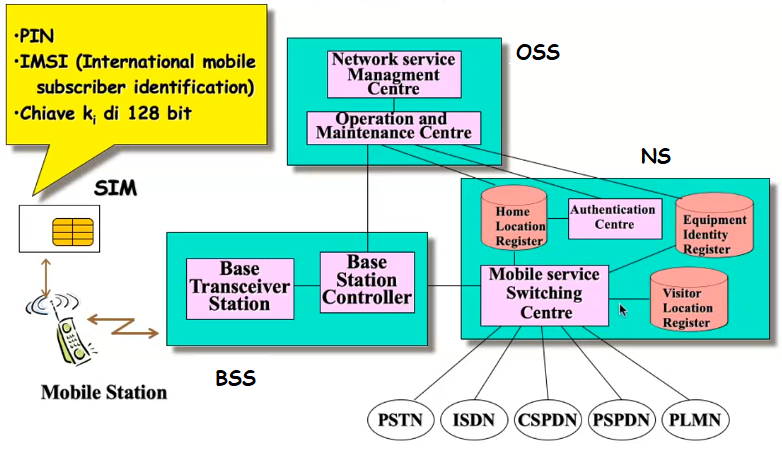
\includegraphics[width=10cm]{./Images/cap1/1.34.png}
\end{figure} 

Vediamo al volo le componenti del sistema GSM:
\begin{itemize}
    \item \textbf{MS (Mobile Station)}: Sistema radio dotato di SIM
    \item \textbf{BSS}: Sottosistema radio comprendente la stazione base. Controlla la trasmissione radio con la MS
    \item \textbf{BTS}: stazione di base con cui la MS comunica
    \item \textbf{BSC}: nodo comune tra le varie BTS
    \item \textbf{NS}: Sottosistema di rete. Realizza la connessione tra l’utente della rete mobile e gli utenti delle altre reti
    \item \textbf{OSS}: Sottosistema di esercizio e manutenzione. Sovraintende al corretto funzionamento della rete
    \item \textbf{NMC}: coordina e gestisce tutti gli OMC presenti nella rete
    \item \textbf{OMC}: responsabile della gestione regionale della rete
    \item \textbf{MSC}: nodo che controlla OSS tutte le BSC in una zona e fornisce la connessione con le reti fisse
    \item \textbf{VLR}: database temporaneo contenente info sulle MS in transito nella zona
    \item \textbf{HLR}: database permanente dei dati di abbonamento degli utenti
    \item \textbf{AuC}: unità che fornisce i dati di autenticazione (IMSI, ki, TMSI, LAI)
    \item \textbf{EIR}: database degli IMEI che identificano le MS
\end{itemize}

Le comunicazioni tra la mobile station e la base station (rete GSM) avvengono con un protocollo che come prima cosa effettua l'autenticazione del dispositivo, dopodiché utilizza una chiave di sessione per stabilire le comunicazioni.
\begin{enumerate}
    \item Mobile Station e Rete GSM posseggono entrambi la chiave \textit{k\textsubscript{i}}.
    \item MS invia una richiesta di accesso a GSM, allegando un \textbf{TMSI} (Temporary Mobile Subscriber Identity), assegnato casualmente dal gestore ad ogni dispositivo mobile nell'area appena questo si accende.
    \item GSM genera un valore casuale a 128 bit e lo invia a MS, il quale utilizza un algoritmo detto A3 dando in input il valore casuale e la propria chiave \textit{k\textsubscript{i}} che produce un valore a 32 bit, che invia a GSM. 
    \item Se questo valore è lo stesso di quello calcolato da GSM con la sua chiave, allora GSM è sicuro dell'identità di MS e l'accesso viene consentito. In questo modo MS e GSM non scambiano informazioni riservate (la chiave) attraverso la tratta radio, evitando così potenziali Replay Attack. Un attacco di questo tipo infatti consisterebbe nel salvare tutti i possibili valori casuali che GSM invia a MS, i quali cambiano in base alla cella e all'orario. Dato che A3 utilizza la chiave privata per inviare la risposta a GSM, ed essendo la chiave privata lunga 128 bit, sappiamo a priori che un attacco di questo tipo non è possibile perché richiede \textit{2\textsuperscript{128}} tentativi.
    \item Una volta avvenuta l'identificazione, GSM genera un altro valore casuale e lo invia a MS, che dà in input ad un algoritmo A8 che restituisce la chiave di sessione \textit{k\textsubscript{c}} a 64 bit. 
    \item La chiave di sessione viene utilizzata per cifrare le informazioni che si scambiano le due parti con un algoritmo A5.
\end{enumerate}

A5 è uno stream cipher usato per cifrare la comunicazione via etere, sottoforma di frame di 114 bit: ogni frame viene identificato da 22 bit e i frame vengono inviati ogni 4.6ms. È una combinazione di 3 LFSR con polinomi di grado 19, 22, 23:
\begin{itemize}
    \item $x^{19} + x^{5} + x^{2} + x + 1$
    \item $x^{22} + x + 1$
    \item $x^{23} + x^{15} + x^{2} + x + 1$
\end{itemize}
La funzione che combina questi registri non è lineare: ad ogni passo ciascun registro viene shiftato se il suo bit centrale concorda con la maggioranza dei bit centrali dei tre registri (0,1,1 $\rightarrow$ shiftano i registri 2 e 3/ 0,1,0 $\rightarrow$ shiftano i registri 1 e 3). In questo modo shiftano almeno due registri ogni round. 

\begin{figure}[htb!]
    \centering
    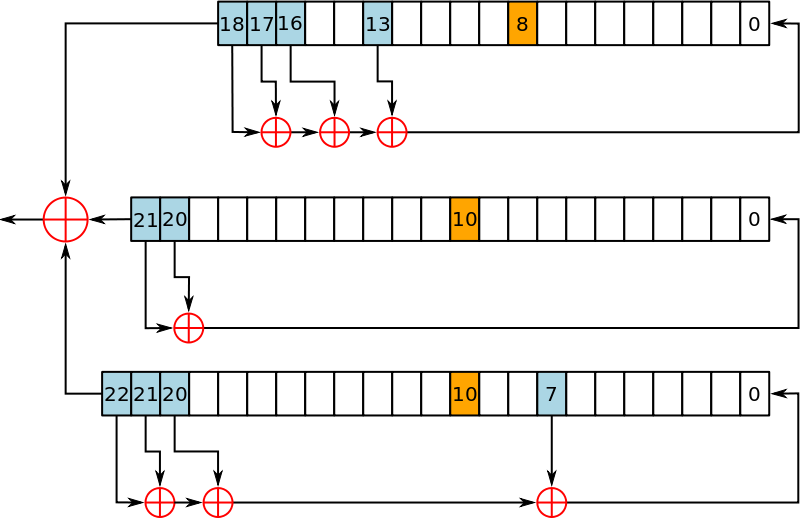
\includegraphics[width=9cm]{./Images/cap1/1.35.png}
\end{figure} 

L'A5 viene inizializzato utilizzando una chiave a 64 bit combinata con un numero di sessione a 22 bit pubblicamente noto. Nelle implementazioni dei campi GSM 10 bit della chiave sono fissati a 0  per cui l'effettiva lunghezza della chiave è di 54 bit. 

\subsection{RC4}
RC4, che prende il nome dal suo ideatore, Ron Rivest (1987) è uno degli stream cipher più conosciuti. Fu tenuto segreto fino al 1994, quando comparve in forma anonima. Il funzionamento di base è semplice: prende in input una chiave e genera un keystream che va in XOR con il testo in chiaro. La chiave ha lunghezza variabile (da 1 a 256 byte), ed è capace di generare keystream con periodo maggiore di \textit{10\textsuperscript{100}}. RC4 è stato implementato in numerosi prodotti, come ad esempio in SSL/TLS per la comunicazione sicura sul web e nello standard IEEE 802.11 WLAN, nella costruzione della chiave WEP.  

L'algoritmo principalmente svolge queste tre operazioni:
\begin{enumerate}
    \item Inizializza il vettore di stato S (permutazione dei 256 byte)
    \item Aggiorna S con la chiave K
    \item Genera la keystream da S
\end{enumerate}
Lo pseudocodice dell'inizializzazione della keystream e per la schedulazione della chiave è il seguente:
\begin{lstlisting}[escapeinside={(*}{*)}]
i,j = 0
while (true)
    i = i + 1 mod 256
    j = (j + S[i]) mod 256
    swap(S[i], S[j])
    t = (S[i] + S[j]) mod 256
    k = S[t]
    
    
j = 0
for i=0 to 255 do
    j = (j + S[i] + K[i mod h]) mod 256
    swap(S[i], S[j])
\end{lstlisting}

Il vettore della chiave è indicato con \texttt{K[0] ... K[h-1]} con \texttt{h} che può essere compreso tra 1 e 256. La fase di inizializzazione riempie il vettore S con una permutazione degli interi da 0 a 255. Dopodiché K viene usata per aggiornare il vettore S, scambiando ciascun \texttt{S[i]} con un \texttt{S[j]}. 

Una volta eseguita l'inizializzazione, viene trovato un valore T che è la somma modulo 256 dei valori \texttt{S[i]} e \texttt{S[j]}, il quale rappresenta l'indice del vettore dove si trova il valore che andrà in input. Il valore del byte k verrà poi messo in XOR con il prossimo byte del testo in chiaro. 

RC4 è stato utilizzato nella crittografia WEP (\textit{Wired Equivalent Privacy}), protocollo in uso fino a qualche anno fa nelle reti WLAN per garantire confidenzialità. Usa una chiave condivisa tra utenti e access point lunga 40 o 104 bit. WEP cifra i pacchetti TCP/IP con RC4 utilizzando un vettore di inizializzazione IV (di 24 bit) che va in input in RC4 e viene inviato in chiaro insieme al pacchetto cifrato. IV viene utilizzato perché altrimenti sarebbe facile per un attaccante rompere il sistema facendo lo XOR tra due pacchetti cifrati e trova informazioni di correlazione dei pacchetti in chiaro. Il pacchetto inviato contiene anche informazioni di checksum per controllarne l'integrità.

\begin{figure}[htb!]
    \centering
    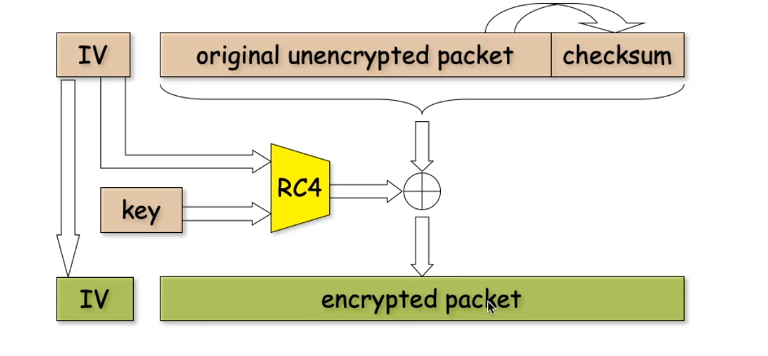
\includegraphics[width=8cm]{./Images/cap1/1.36.png}
\end{figure} 

\subsubsection{\textbf{ATTACCHI AL WEP}}
Il primo attacco eseguito con successo al WEP è avvenuto nel 2001 e la vulnerabilità non era in RC4 bensì nella generazione della chiave in input a RC4, infatti IV veniva inviato in chiaro. Furono poi proposte delle modifiche a WEP per rendere vano l'attacco. Un secondo tipo di attacco avvenne nel 2007, quando si riuscì a rompere il WEP a 104 bit in meno di un minuto, perché l'attaccante che riusciva ad ottenere un numero molto alto di pacchetti cifrati aveva una probabilità molto alta di trovare pacchetti cifrati con lo stesso vettore di inizializzazione e quindi riusciva facilmente a rompere lo schema (40.000 pacchetti, probabilità successo 50\%, 85.000 pacchetti, probabilità successo 95\%). 

In rete si trovano diverse suite di software che permettono di verificare la sicurezza delle proprie chiavi WEP eseguendo attacchi di questo tipo. Dopo il WEP sono stati implementati diversi protocolli di sicurezza WLAN, tra cui WPA, WPA2 e WPA3, tutti grazie all'organizzazione no-profit Wi-Fi Alliance.

\begin{itemize}
    \item \textbf{WPA}
    \begin{itemize}
        \item Intermedio, per evitare i problemi di sicurezza del WEP
        \item Usa Temporal Key Integrity Protocol (TKIP) per mischiare chiave
        \item Implementabile come upgrade firmware
    \end{itemize}
    \item \textbf{WPA2}
    \begin{itemize}
        \item AES e Counter Mode CBC-MAC Protocol (CCMP)
    \end{itemize}
    \item \textbf{WPA3}
    \begin{itemize}
        \item WPA3-Enterprise: AES-256 in Galois/Counter Mode (GCM)
mode ed HMAC con SHA-384
        \item WPA3-Personal: AES-128 in Counter with CBC-MAC (CCM) mode
        \item Forward secrecy, ovvero se l'attaccante riceve informazioni sulla cifratura oggi, ciò non compromette i pacchetti scambiati in passato, anche se sono posseduti dall'attaccante. 
    \end{itemize}
\end{itemize}

RC4 veniva utilizzato anche in altri protocolli, come BitTorrent (viene scartato il primo kilobyte per prevenire attacchi come il precedente), Skype, Kerberos, PDF, Secure Shell (SSH), ma in seguito all'esposizione di vulnerabilità è stato abbandonato a favore di altri protocolli, come AES. 

\subsection{Salsa20}
È uno stream cipher proposto nel 2005 con chiave a 128 o 256 bit. Ha un nonce/vettore di inizializzazione di 64 bit. È basato su operazioni ARX (add-rotate-xor) su 32 bit, quindi facilmente implementabili su architetture a 32 bit perché basta ignorare i riporti e prendere i 32 bit meno significativi. la funzione principale utilizzata che viene ripetuta più volte a seconda dei round è:

\[R(a,b,c,k) = b \oplus b \oplus ((a \boxplus c) <<< k) \]

Questa funzione viene eseguita in diversi round. Il numero di round di solito è 20 ed è possibile ridurli: in questo caso si fa riferimento a Salsa20/12 e Salsa20/8. Riducendo il cifrario diminuisce il livello di sicurezza ma anche il livello di complessità. 

\begin{figure}[htb!]
    \centering
    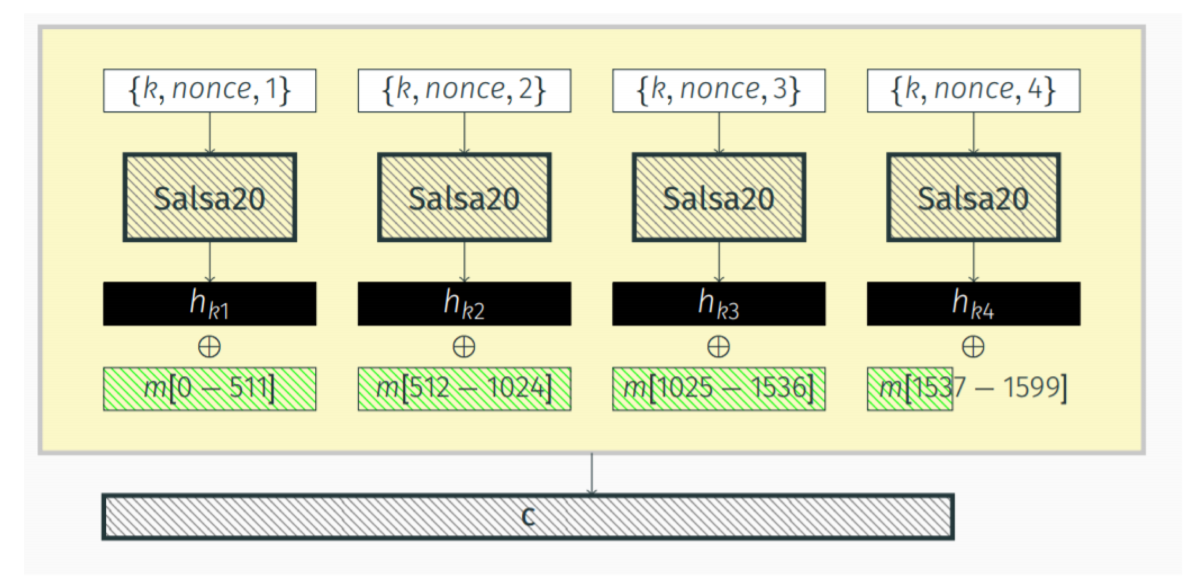
\includegraphics[width=9cm]{./Images/cap1/1.37.png}
\end{figure} 

Il funzionamento è simile a quello degli altri stream cipher: la stringa di valori viene generata secondo un algoritmo e messa in XOR con il testo in chiaro. Il testo in chiaro nell'immagine è rappresentato dal vettore m, diviso in parti da 512 bit.

Ogni parte \textit{i} costruisce una stringa con un algoritmo a cui da in input la chiave, il vettore di inizializzazione, e il valore \textit{i}. Per decifrare il testo, basta utilizzare la stessa identica struttura, dividendo il testo cifrato in parti da 512 bit e applicando lo stesso algoritmo. 

\vspace{5mm}

Salsa20 opera su uno stato di 512 bit, organizzati in 16 word di 32 bit, organizzate in una matrice. Lo stato iniziale della matrice è organizzato come l'immagine seguente:

\begin{figure}[htb!]
    \centering
    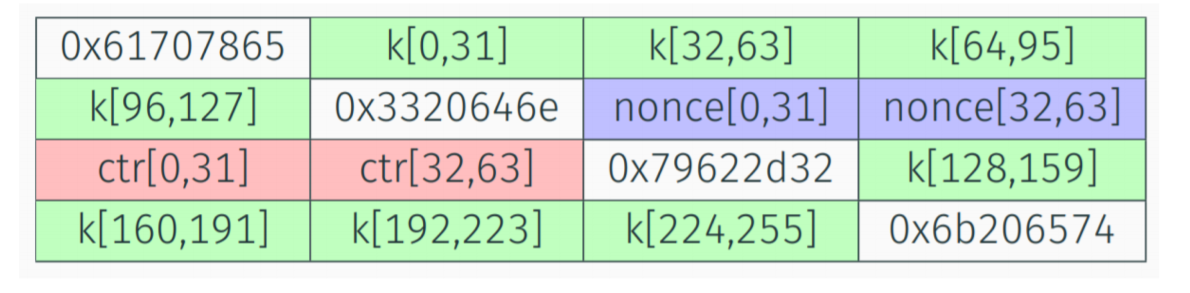
\includegraphics[width=11cm]{./Images/cap1/1.38.png}
\end{figure} 

\begin{itemize}
    \item 8 celle sono occupate dalla chiave (\textit{8x32 = 256} bit);
    \item 4 posizioni nella diagonale principale sono occupate da una costante: \textit{"expand 32-byte k"} in ASCII.
    \item 2 parole sono occupate dal vettore di inizializzazione.
    \item 2 posizioni rappresentano il numero del blocco a cui appertengono. Essendo due parole da 32 bit, posso avere un numero di blocchi da 512 bit pari a 2\textsuperscript{64}.
\end{itemize}
Le operazioni vengono effettuate prima su ogni colonna e poi su ogni riga. In pseudocodice:
\begin{lstlisting}
for round = 1 to 10 do
    quarterround(x[0], x[4], x[8], x[12])
    quarterround(x[5], x[9], x[13], x[1])
    quarterround(x[10], x[14], x[2], x[6])
    quarterround(x[15], x[3], x[7], x[11])
for round = 1 to 10 do
    quarterround(x[0], x[1], x[2], x[3])
    quarterround(x[5], x[6], x[7], x[4])
    quarterround(x[10], x[11], x[8], x[9])
    quarterround(x[15], x[12], x[13], x[14])
\end{lstlisting}
Dal numero di round deriva anche il nome dell'algoritmo. L'operazione di \textit{quarterround} è specificata in questa immagine, dove possiamo vedere l'addizione mod 32, lo XOR e la rotazione a sinistra:

\begin{figure}[htb!]
    \centering
    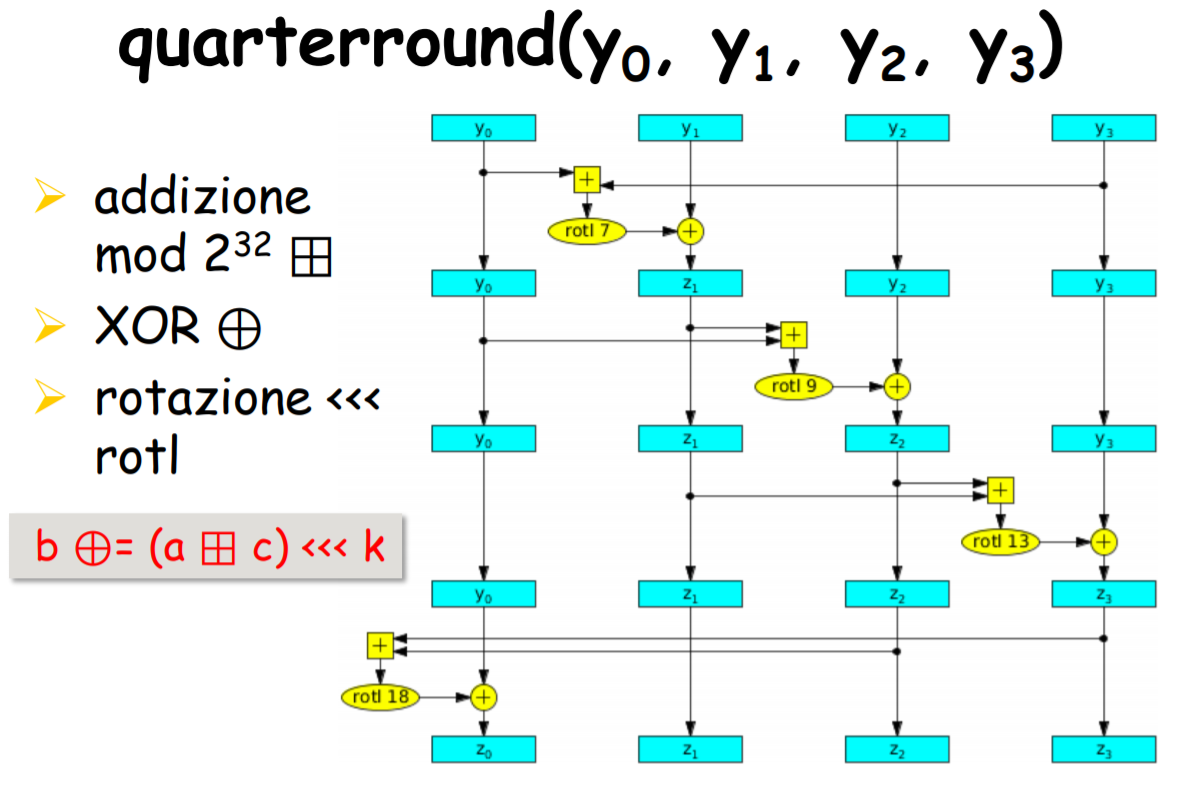
\includegraphics[width=11cm]{./Images/cap1/1.39.png}
\end{figure} 

\subsection{ChaCha20}
ChaCha20 è un algoritmo proposto nel 2008, la cui funzione primitiva è:

\[ b = b \boxplus c\]
\[a = a \oplus b\]
\[a = a \lll k\]

Anche ChaCha20 possiede una matrice di stato, il cui stato iniziale ha la stessa struttura del Salsa20 ma in posizioni diverse:

\begin{figure}[htb!]
    \centering
    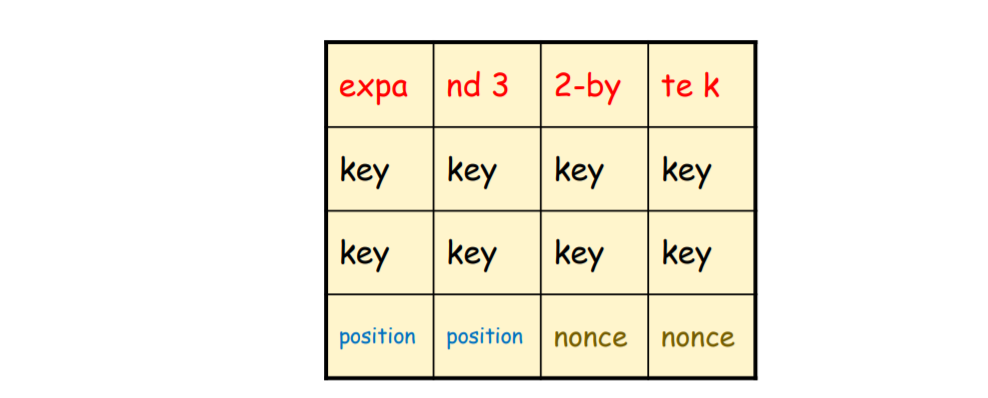
\includegraphics[width=8cm]{./Images/cap1/1.40.png}
\end{figure} 

La sequenza delle operazioni in pseudocodice è la stessa del Salsa20 per quanto riguarda le colonne, cambia solamente l'operazione primitiva. La seconda parte anzichè agire sulle righe agisce sulle diagonali (0,5,10,15), (1,6,11,12), (2,7,8,13), (3,4,9,14). 

L'algoritmo ChaCha20 è stato selezionato per sostituire l'RC4 in TLS e openSSL.

\subsection{Accenni a TLS e SSL}
L'ultima versione di TLS attualmente è la 1.3 di agosto 2018. Nel changelog c'è una voce che indica che è stato aggiunto ChaCha20 e che è vietato utilizzare implementazioni di RC4 a causa delle sue vulnerabilità. SSL è un protocollo di sicurezza sviluppato da Netscape e ancora molto diffuso nella sua versione 3. SSL si trova sopra il protocollo TCP/IP e sotto il protocollo di applicazione. 

\begin{figure}[htb!]
    \centering
    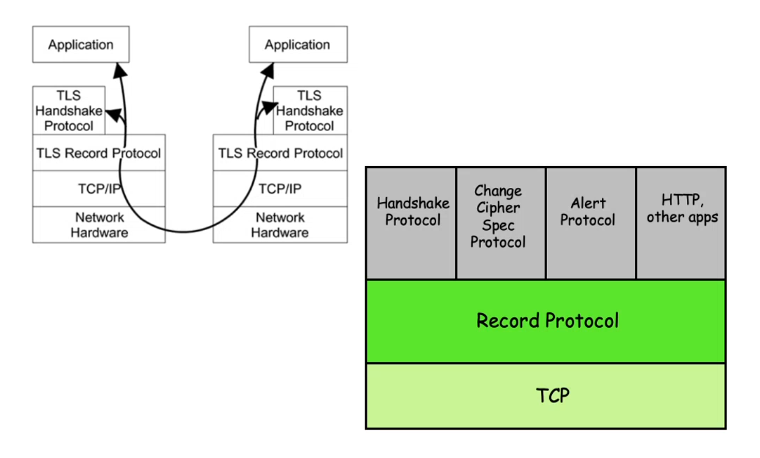
\includegraphics[width=9cm]{./Images/cap1/1.41.png}
\end{figure} 

La parte del Record Protocol riceve i dati dal blocco superiore e li divide in blocchi, comprimendoli eventualmente. Dopodiché calcola il MAC, cifra i blocchi e trasmette il risultato. TLS viene utilizzato da client e server, e in particolare ne viene utilizzato il protocollo handshake, per:
\begin{itemize}
    \item negoziare ciphersuite (quali sono gli algoritmi che saranno utilizzati);
    \item autenticazione;
    \item stabilire le chiavi da usare nel Record Protocol.
\end{itemize}
Il RP fornisce confidenzialità e autenticità. Nella versione 1.3 di TLS sono stati rimossi diversi algoritmi obsoleti, come RC4, DES, 3DES, AES-CBC, MD5 e SHA-1. Esistono diversi siti che eseguono una verifica dei protocolli di sicurezza, tra cui \textbf{Cloudflare} e \textbf{How's My SSL}. 

\begin{figure}[htb!]
    \centering
    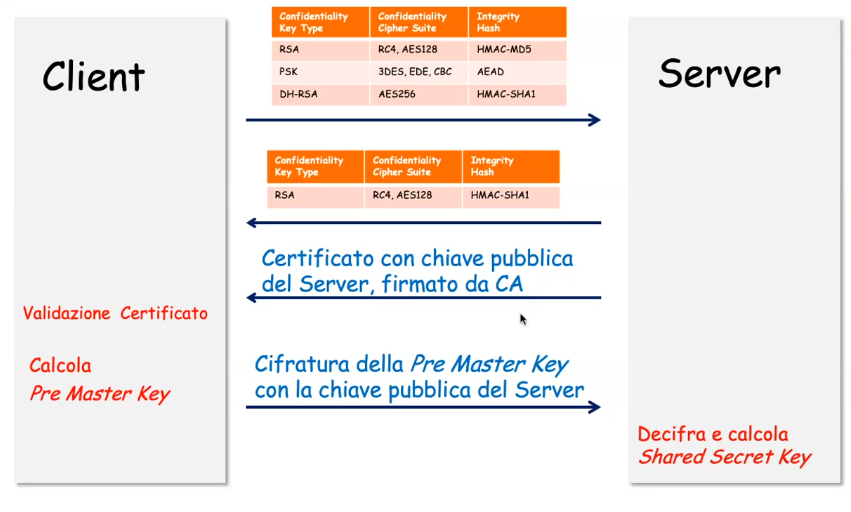
\includegraphics[width=9cm]{./Images/cap1/1.42.png}
\end{figure} 

\section{Crittografia a chiave pubblica}
La gestione delle chiavi nella crittografia a chiave privata è complicata in quanto in una rete con \textit{n} utenti ogni coppia di utenti deve condividere una chiave, per cui ogni utente deve memorizzare \textit{n-1} chiavi. Il numero totale delle chiavi segrete è $\frac{n(n-1)}{2}$. Inoltre l'aggiunta di un nuovo utente alla rete implica la distribuzione della chiave a tutti i precedenti utenti.

La crittografia a chiave pubblica (o asimmetrica) si basa su due chiavi: una pubblica che cifra il messaggio e una privata che decifra il messaggio. Gli utenti devono solamente condividere la chiave pubblica.

I cifrari asimmetrici si basano su funzioni dette \textit{one way}, ovvero facili da calcolare e difficili da invertire. Con difficili come al solito indichiamo funzioni non polinomiali, quindi esponenziali o subesponenziali.


\begin{comment}
\subsection{Elementi di Teoria dei numeri}
\subsubsection{\textbf{ARITMETICA MODULARE}}
\subsubsection{\textbf{ALGORITMO DI EUCLIDE PER IL CALCOLO DEL GCD}}
\subsubsection{\textbf{CALCOLO DELL'INVERSA MOLTIPLICATIVA MOD N}}
\subsubsection{\textbf{ELEVAZIONE A POTENZA MODULARE}}
\subsubsection{\textbf{GENERAZIONE DI NUMERI PRIMI}}
\subsubsection{\textbf{TEST DI PRIMALITÀ}}
\end{comment}
 

\subsection{RSA}
Il primo algoritmo a chiave pubblica che ebbe successo fu RSA, proposto nel 1978 da \textbf{R}ivest, \textbf{S}hamir e \textbf{A}dleman. Supponiamo che le chiavi siano due coppie: \textit{(n, e)} la chiave pubblica, e \textit{(n, d)} la chiave privata. Il valore \textit{n} viene generato come prodotto di due numeri \textit{p} e \textit{q}, entrambi primi. I valori \textit{e} e \textit{d} sono tali che $e \dot d = 1$ \texttt{mod} $(p-1)(q-1)$. 
Per inviare un messaggio ad Alice, Bob cifra il messaggio utilizzando la funzione \textit{C $\rightarrow$ M\textsuperscript{e} mod n}. Per decifrare il messaggio, Alice trova il messaggio utilizzando la funzione \textit{M $\rightarrow$ C\textsuperscript{d} mod n}. 

La correttezza della cifratura RSA può essere vista in questo modo:

\begin{equation}
\begin{split}
C^{d} \mod n & = (M^{e})^{d} \mod n\\
 & = M^{ed} \mod n\\
 & = M^{1+k(p-1)(q-1)} \mod n\\
 & = M \dot (M^{(p-1)(q-1)})^{k}\\
 & = M \mod n\\
 & = M
\end{split}
\end{equation}
L'ultima uguaglianza è data dal fatto che $0\leq M < n$. 

RSA utilizza le seguenti computazioni:
\begin{itemize}
    \item generazione numeri primi \textit{p} e \textit{q}, molto grandi
    \item generazione di \textit{d} ed \textit{e}:
    \begin{itemize}
        \item generazione di e (\textit{e} e \textit{d} sono relativamente primi rispetto alla funzione di Eulero di \textit{n}).
        \item $d \leftarrow e^{-1} \mod (p-1)(q-1)$
    \end{itemize}
    \item elevazione a potenza modulare (per cifratura e decifratura)
\end{itemize}
L'elevazione a potenza modulare (ovvero \textit{x\textsuperscript{y} mod z}) può essere calcolata con tre metodi differenti: metodo naive, metodo left-to-right e metodo right-to-left.
Il primo metodo, come suggerisce il nome, è illustrato di seguito:
\begin{lstlisting}[escapeinside={(*}{*)}]
potenza_modulare_naive(x,y,z)
    a (*$\leftarrow$*) 1
    for i = 1 to y do
        a (*$\leftarrow$*) (a (*$\times$*) x) mod z
    return a
\end{lstlisting}
La complessità è proporzionale a \textit{y}, per cui se \textit{y} è di 1024 bit, occorrono circa 2\textsuperscript{1024} operazioni. L'algoritmo è esponenziale nella lunghezza dell'esponente, quindi diventa inutilizzabile. Serve infatti un algoritmo proporzionale a 1024, non a 2\textsuperscript{1024}. Si considera allora la rappresentazione binaria di \textit{y}, seguendo uno dei due metodi left-to-right o right-to-left, in base a se vado dal coefficiente più significativo a quello significativo dell'esponente o viceversa. Questi metodi hanno complessità lineare rispetto alla lunghezza dell'esponente.

\begin{figure}[htb!]
    \centering
    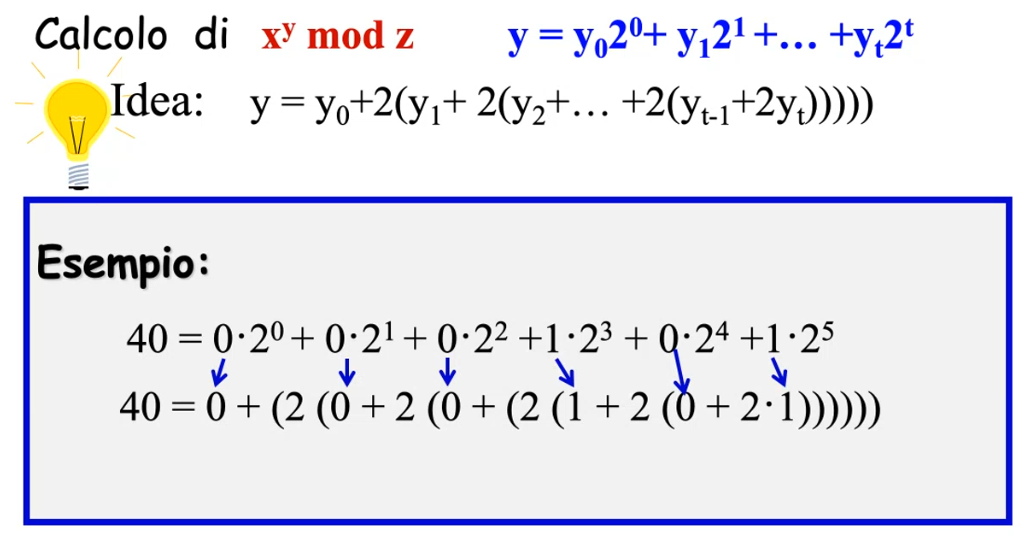
\includegraphics[width=10cm]{./Images/cap1/1.43.png}
\end{figure} 

L'idea è quella di mettere a fattore sempre 2 a ogni valore, mettendo da parte il valore meno significativo della parte rimanente. Nell'immagine è rappresentata questa operazione. Una volta calcolato questo valore, devo elevare \textit{x} a questo valore (dato che devo calcolare \textit{x\textsuperscript{y}}). Acendo una somma nell'esponente posso quindi semplificare e portare fuori, come mostrato dall'immagine successiva.

\begin{figure}[htb!]
    \centering
    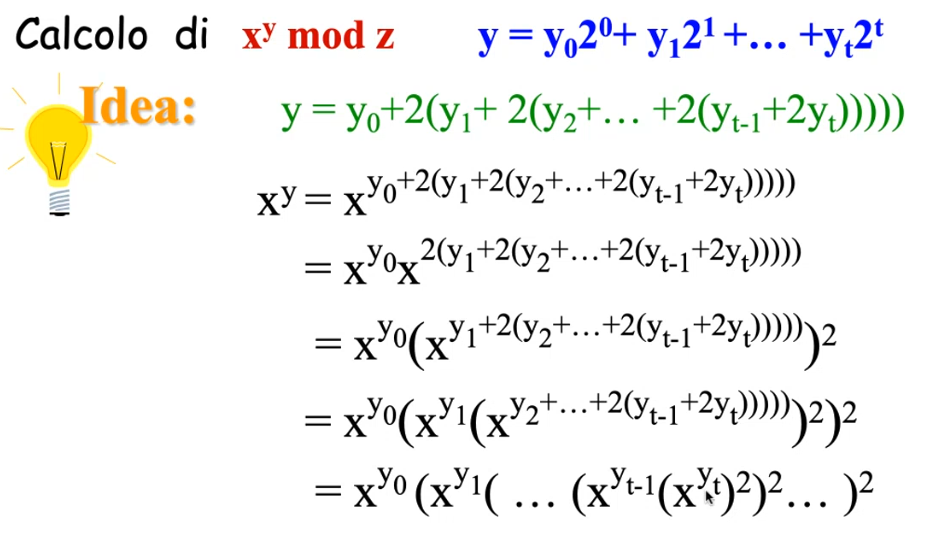
\includegraphics[width=10cm]{./Images/cap1/1.44.png}
\end{figure} 

E quindi alla fine risulta, come si può vedere di seguito, che l'algoritmo parte dalle parentesi più interne ed esegue il quadrato, dopodiché moltiplica per x oppure non moltiplica, poi riesegue il quadrato e così via.
 
\begin{figure}[htb!]
    \centering
    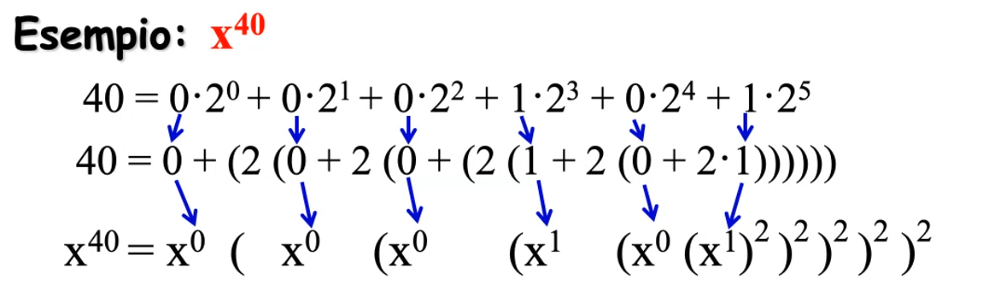
\includegraphics[width=10cm]{./Images/cap1/1.45.png}
\end{figure} 

In questo modo il numero di cicli effettuati è polinomiale sulla lunghezza dell'esponente:
\begin{lstlisting}[escapeinside={(*}{*)}]
potenza_modulare(x,y,z)
    a (*$\leftarrow$*) 1
    for i = t downto 0 do
        a (*$\leftarrow$*) (a (*$\times$*) a) mod z
        if (*$y_{i}$*) = 1 then
             a (*$\leftarrow$*) (a (*$\times$*) x) mod z
    return a
\end{lstlisting}

Il secondo metodo utilizza un metodo alternativo di rappresentazione dell'esponente:

\begin{figure}[htb!]
    \centering
    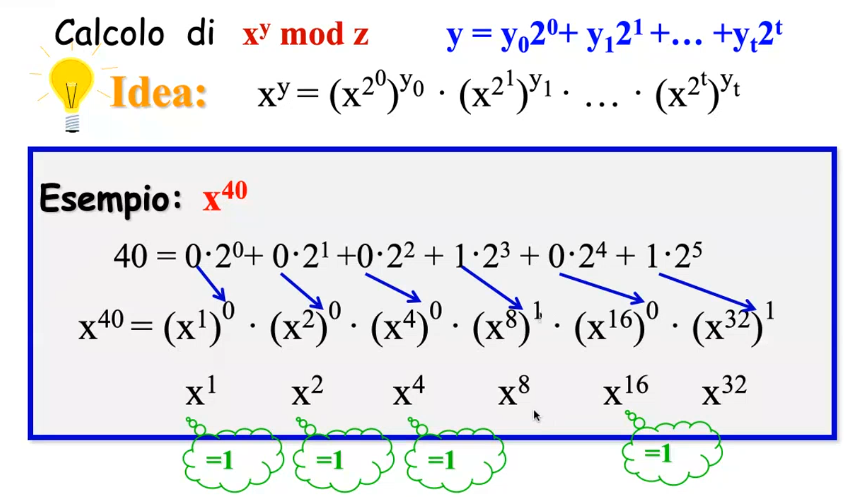
\includegraphics[width=10cm]{./Images/cap1/1.46.png}
\end{figure} 

In questo modo è l'esponente esterno a cambiare e non quello dentro la parentesi. Gli esponenti sono tutte potenze di 2, per cui ogni valore è calcolabile facilmente da quello precedente, moltiplicando quel valore per sé stesso. Questo algoritmo è il più semplice da implementare, ed è sempre polinomiale nella lunghezza dell'esponente:
\begin{lstlisting}[escapeinside={(*}{*)}]
potenza_modulare(x,y,z)
    if y = 0 then
        return 1
    X (*$\leftarrow$*) x
    P (*$\leftarrow$*) 1
    for i = 1 to t do
        X (*$\leftarrow$*) (X (*$\times$*) X) mod z
        if (*$y_{i}$*) = 1 then
             P (*$\leftarrow$*) (P (*$\times$*) X) 
\end{lstlisting}
Per calcolare velocemente l'elevamento a potenza modulare si può utilizzare anche la formula di Garner:

\[ x^{y} \mod n = q (q^{-1} (a-b) \mod p) + b\]

dove $a = x^{y} \mod p$ e $b = x^{y} \mod q$. Ricordiamo che in RSA \textit{n} è un numero composto, prodotto di due primi \textit{p} e \textit{q}, per cui svolgere separatamente le operazioni modulo \textit{p} e \textit{q} è più efficiente rispetto ad \textit{n}.

La scelta dei numeri primi molto grandi avviene in un modo semplice con un algoritmo probabilistico: 
\begin{enumerate}
    \item Viene generato a caso un numero dispari \textit{p} di grandezza appropriata.
    \item Viene testato se \textit{p} è primo.
    \item Se \textit{p} è composto, torna al punto 1.
\end{enumerate}
Ogni volta che viene fatto un ciclo, la probabilità di trovare un numero prima dipende dal numero di numeri primi della grandezza specificata. La media dell'algoritmo è l'inverso della probabilità di successo, quindi se ad ogni iterazione ho probabilità \textit{1/n} di trovare un numero primo, in media l'algoritmo farà \textit{n} iterazioni. L'efficienza dell'algoritmo quindi dipende principalmente dal numero di numeri primi che posso trovare data una grandezza: se è molto piccolo allora l'algoritmo necessità di molti passi per trovarne uno; viceversa con un numero grande di numeri primi sarà più semplice. Secondo il teorema dei numeri primi, il numero di numeri primi nell'intervallo $[2,x]$ è 

\[\pi (x) \approx \frac{x}{\ln x}\]

La scelta di un primo numero di 512 bit ad esempio, implica che il primo e l'ultimo bit siano 1 (perchè la lunghezza deve essere esattamente 512 bit e per avere numeri dispari) e che i 510 bit centrali siano scelti a caso. La probabilità di trovare un numero primo è:

\[\frac{\text{\#primi in}[2^{511},2^{512}-1]}{\text{\#numeri in insieme}} \approx \frac{\frac{2^{512}}{\ln 2^{512}} - \frac{2^{511}}{\ln 2^{511}}}{2^{510}} \approx \frac{1}{177,79}\]

Questo significa che il numero medio di tentativi per trovare un numero primo è 177,79 (nel caso di 1024 bit, il numero di tentativi è il doppio). Il problema ora è che la complessità dell'algoritmo dipende dal modello di test del numero trovato: infatti non posso fattorizzare il numero trovato e vedere se i fattori primi sono solo 1 e sé stesso, perché sappiamo che non esistono algoritmi efficienti per il calcolo della fattorizzazione. Per testare che il numero trovato è primo allora possiamo contare su due tipi di algoritmi: probabilistici e deterministici. 
\begin{itemize}
    \item Nel primo caso il test può sbagliare, potrebbe infatti dichiarare primo un numero composto. Nel caso in cui il numero sia composto invece l'algoritmo non commette errori. Se un numero viene dichiarato primo, posso ripetere il test con lo stesso numero \textit{t} volte per avere probabilità 1/2\textsuperscript{t}. I due algoritmi più utilizzati sono il Test di Solovay-Strassen, con probabilità di errore $\leq$ \textit{1/2\textsuperscript{t}}, e il Test di Miller-Rabin, più veloce e più usato, con probabilità di errore $\leq$ \textit{1/4\textsuperscript{t}}.
    \item Per quanto riguarda i test deterministici, non erano noti algoritmi efficienti fino al 2002, quando fu proposto il test deterministico AKS, con complessità \textit{O(log\textsuperscript{6} n)}. Tuttavia viene ancora usato Miller-Rabin perché è più efficiente.
\end{itemize}

\vspace{5mm}

La generazione delle chiavi di RSA segue questo algoritmo:
\begin{lstlisting}
1.  input L
2.  genera 2 primi di lunghezza L/2
3.  n = p * q
4.  scegli a caso e 
5.  if (gcd(e,(p-1)(q-1))) = 1 then
      d = 1/e mod (p-1)(q-1)
6.  else
      goto 4
\end{lstlisting}
I numeri primi vengono scelti con lunghezza esattamente la metà di L perché la sicurezza di RSA si basa sul fatto che \textit{n} è difficile da fattorizzare, quindi valori della stessa grandezza rendono ancora più difficile la fattorizzazione. Tuttavia l'algoritmo RSA funzionerebbe lo stesso anche con lunghezze diverse. Il passo 5 controlla se \textit{e} e \textit{(p-1)(q-1)} sono relativamente primi. Si può fare un miglioramento su \textit{e}, in quanto deve essere pubblico: si può scegliere in modo da minimizzare le operazioni di cifratura. In genere o l'esponente viene scelto come 3, essendo molto semplice, oppure 2\textsuperscript{16}-1, in decimale 65537, in binario 10000000000000001. Questo valore di \textit{e} è abbastanza piccolo, quindi il ciclo varia solo su 16 valori. Inoltre in questo modo il calcolo di M\textsuperscript{e} richiede solo 16 quadrati ed una moltiplicazione. Non conviene comunque scegliere forzatamente \textit{e} al passo 6 perché potrebbe non essere relativamente primo con \textit{(p-1)(q-1)} quindi potrebbe ciclare all'infinito. Può però essere usata questa variante:
\begin{lstlisting}
1.  input L
2.  e = 3 oppure e = 65537
3.  genera 2 primi di lunghezza L/2
4.  n = p * q
5.  if (gcd(e,(p-1)(q-1))) = 1 then
      d = 1/e mod (p-1)(q-1)
6.  else
      goto 3
\end{lstlisting}
Controlliamo la sicurezza della generazione delle chiavi di RSA. Un attaccante conoscendo la chiave pubblica \textit{(n,e)} vorrebbe calcolare la chiave privata \textit{d = e\textsuperscript{-1} mod (p-1)(q-1)}. Se l'attaccante potesse fattorizzare \textit{n}, saprebbe computare \textit{d}, perché potrebbe calcolare \textit{(p-1)(q-1)}. Ma anche se sapesse computare \textit{(p-1)(q-1)} saprebbe fattorizzare \textit{n}, utilizzando un semplice sistema di equazioni. Anche se potesse computare \textit{d} saprebbe fattorizzare \textit{n}, infatti un algoritmo che trova \textit{d} con input \textit{(n,e)} può essere usato come oracolo in un algoritmo Las Vegas che fattorizza \textit{n} con probabilità $\geq$ 1/2. Al momento però l'algoritmo più veloce per la fattorizzazione è il General Number Field Sieve, con complessità sub-esponenziale. 

L'equivalenza per la sicurezza tra le lunghezze delle chiavi pubbliche e simmetriche si stabilisce risolvendo l'equazione:

\[2^{k} = \text{complessità GNFS} (2^{N})\]

dove \textit{2\textsuperscript{k}} rappresenta la sicurezza di un cifrario a blocchi con chiave di \textit{k} bit e la complessità \textit{GNFS} rappresenta la sicurezza RSA per \textit{n} di lunghezza \textit{N = log\textsubscript{2} n}.

\subsubsection{Sicurezza di RSA}
L'attaccante conosce la chiave pubblica \textit{(n,e)} e il messaggio cifrato \textit{C = M\textsuperscript{e} mod n} e vuole calcolare il messaggio \textit{M}. Il problema è che attualmente il migliore algoritmo per rompere RSA consiste nel fattorizzare e poi trovare \textit{M}, ma non si sa se queste due cose siano equivalenti. Degli attacchi non basati su questo problema sono chosen ciphertext attack, common modulus attack e low exponent attack. RSA è sensibile ad attacchi CCA a causa delle proprietà di omomorfismo: conoscendo due cifrati e un messaggio in chiaro, è possibile trovare il messaggio in chiaro mancante:

\[(M_{1} \times M_{2})^{e} = M_{1}^{e} \times M_{2}^{e} = C_{1} \times C_{2} \mod n\]

\begin{figure}[htb!]
    \centering
    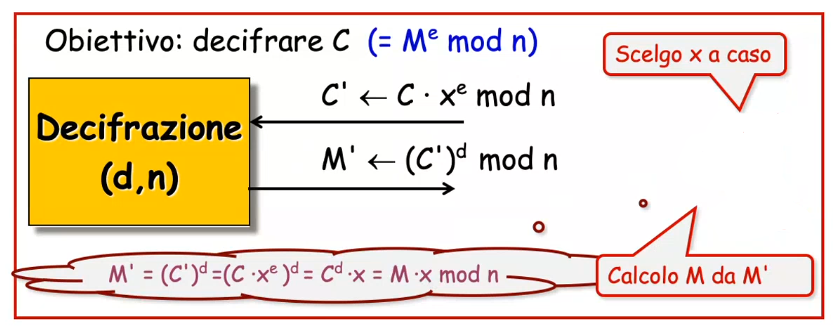
\includegraphics[width=11cm]{./Images/cap1/1.47.png}
\end{figure} 

Altri attacchi a cui è sensibile RSA sono:
\begin{itemize}
    \item \textbf{Timing attack}: ricava i bit di \textit{d}  uno alla volta, analizzando il tempo richiesto per l'esponenziazione modulare (decifratura);
    \item \textbf{Power attack}: ricava \textit{d} analizzando la potenza consumata da una smartcard durante la decifratura. 
\end{itemize}
Contromisure a questi attacchi sono applicare un ritardo costante, in modo che tutte le esponenziazioni richiedano lo stesso tempo, un ritardo casuale, introducendo quindi un "rumore" per confondere l'avversario, e il blinding, ovvero moltiplicare il cifrato per un numero casuale prima di decifrare.

\begin{mdframed}[backgroundcolor=gray!20,shadow=false]
\textbf{Q: Quando usare la crittografia a chiave privata e quando quella a chiave pubblica?}

A: La crittografia a chiave pubblica è utile perché le chiavi private non vengono mai trasmesse ed è possibile la firma digitale. La crittografia a chiave privata è molto più veloce ed efficiente di quella a chiave pubblica, ed è sufficiente in situazioni di non scalabilità, ad esempio in applicazioni per singolo utente.
\end{mdframed}

Normalmente la crittografia a chiave pubblica viene utilizzata per cifrare una chiave di sessione, la quale funge da chiave privata per la vera e propria cifratura. Questo principalmente perché la crittografia a chiave privata è più veloce ma non si vuole rinunciare ai benefici della chiave pubblica come la necessità di non scambiarsi le chiavi. Tuttavia nel caso di applicazioni semplici è molto facile riuscire a rompere RSA, per cui fa effettuato un preprocessing prima di cifrare il messaggio. I due modi per effettuare il preprocessing sono stati definiti nello standard PKCS1, che rende casuale il messaggio da cifrare con gli schemi RSAES-PKCS1-v1.5 e RSAES-OAEP (Optimal Asymmetric Encryption Padding). Il primo cifra il valore mostrato di seguito:

\begin{figure}[htb!]
    \centering
    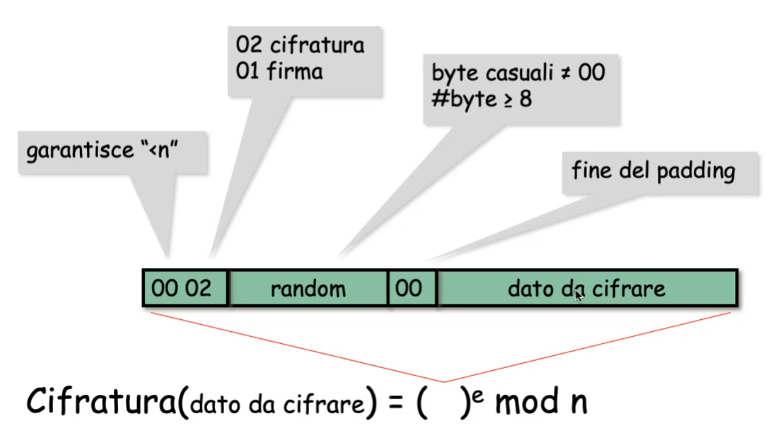
\includegraphics[width=10cm]{./Images/cap1/1.48.png}
\end{figure} 

Questo schema ha avuto dei problemi di sicurezza nel passato perché sensibile ad attacchi CCA. Il secondo metodo di cifratura, OAEP, assomiglia ad un cifrario Feistel, e si prepone di mascherare il formato del messaggio da cifrare, quindi è più sicuro rispetto a PKCS1.

\begin{figure}[htb!]
    \centering
    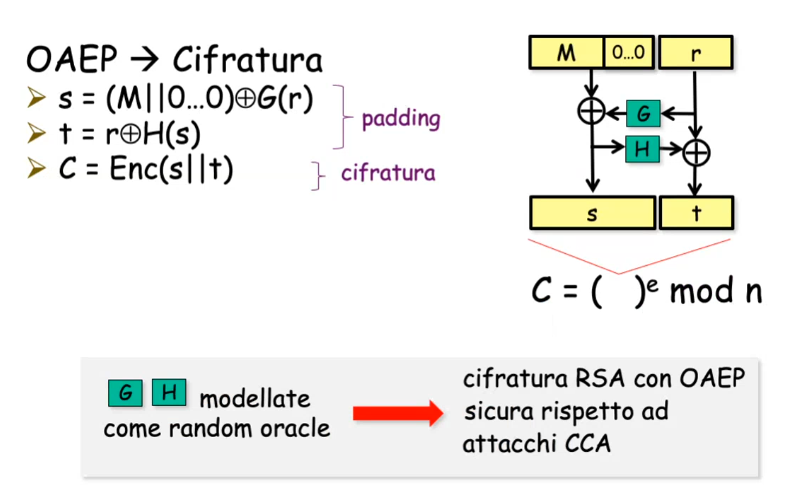
\includegraphics[width=9cm]{./Images/cap1/1.49.png}
\end{figure} 

Per decifrare un messaggio cifrato con OAEP basta applicare le operazioni in ordine inverso, tenendo conto degli 0 di padding aggiunti alla fine del messaggio.

\begin{figure}[htb!]
    \centering
    \includegraphics[width=10cm]{./Images/cap1/1.50.png}
\end{figure} 

Questo è lo standard che viene effettivamente utilizzando quando viene utilizzato RSA. 

\subsection{Accordo su chiavi}
L'accordo sulle chiavi da scambiarsi per le due parti può avvenire secondo gli schemi di Diffie-Hellman utilizzando gli insiemi \textit{Z\textsubscript{p}}. Vengono anche utilizzate tecniche che comprendono il logaritmo discreto, con algoritmi quali trial multiplication e index calculus. Il migliore algoritmo conosciuto per rompere Diffie-Hellman  calcola prima il logaritmo discreto e poi trova il valore dell'esponente. Come nel caso precedente, la complessità è sub-esponenziale. Questo protocollo è sicuro contro attacchi passivi ma non contro attacchi man-in-the-middle, a meno che non si utilizzi l'autenticazione. Inoltre potrebbe essere anche usato come cifrario asimmetrico, ma RSA viene utilizzato per motivi commerciali e storiche.

Lo scambio di chiavi Diffie-Hellman (in inglese Diffie-Hellman key exchange) è un protocollo crittografico che consente a due entità di stabilire una chiave condivisa e segreta utilizzando un canale di comunicazione insicuro (pubblico) senza la necessità che le due parti si siano scambiate informazioni o si siano incontrate in precedenza. La chiave ottenuta mediante questo protocollo può essere successivamente impiegata per cifrare le comunicazioni successive tramite uno schema di crittografia simmetrica.

Sebbene l'algoritmo in sé sia anonimo (cioè non autenticato) è alla base di numerosi protocolli autenticati ed è usato anche in alcune modalità di funzionamento del protocollo TLS.

\vspace{5mm}

Nell'implementazione originale (e più semplice) del protocollo si considera inizialmente un numero g, generatore del gruppo moltiplicativo degli interi modulo p, dove p è un numero primo. Uno dei due interlocutori, ad esempio Alice, sceglie un numero casuale "a" e calcola il valore A = g\textsuperscript{a} mod p (dove mod indica l'operazione modulo, ovvero il resto della divisione intera) e lo invia attraverso il canale pubblico a Bob (l'altro interlocutore), assieme ai valori g e p. Bob da parte sua sceglie un numero casuale "b" , calcola B = g\textsuperscript{b} mod p e lo invia ad Alice. A questo punto Alice calcola K\textsubscript{A} = B\textsuperscript{a} mod p, mentre Bob calcola K\textsubscript{B} = A\textsuperscript{b} mod p.
I valori calcolati sono gli stessi, in quanto B\textsuperscript{a} mod p = A\textsuperscript{b} mod p.
A questo punto i due interlocutori sono entrambi in possesso della chiave segreta e possono cominciare ad usarla per cifrare le comunicazioni successive.
Un attaccante può ascoltare tutto lo scambio, ma per calcolare i valori a e b avrebbe bisogno di risolvere l'operazione del logaritmo discreto, che è computazionalmente onerosa e richiede parecchio tempo, in quanto sub-esponenziale (sicuramente molto più del tempo di conversazione tra i 2 interlocutori).

\vspace{5mm}

Purtroppo l'algoritmo Diffie-Hellman è vulnerabile all'attacco "Man in the middle", durante il quale un agente terzo può falsificare le chiavi pubbliche di Alice e Bob ed ingannare le due parti. L'algoritmo infatti attua lo scambio delle chiavi simmetriche segrete, ma con il presupposto di avere delle informazioni pubbliche condivise e si dimostra resistente nei confronti dell'intercettamento di queste ultime (a partire dalle informazioni pubbliche non si riesce a ricostruire la chiave, è computazionalmente difficile). Ma nulla può impedire che le informazioni pubbliche siano state modificate o falsificate; in questo caso Alice e Bob non avrebbero modo di accorgersi della frode appoggiandosi al solo algoritmo Diffie-Hellman. Ecco perché occorre che le informazioni pubbliche, ovvero le chiavi p e g degli esempi, possano essere autenticate tramite un algoritmo di autenticazione o da un Certification Authority.

Una variante del protocollo è DH-EKE, facente parte della famiglia Encrypted Key Exchange, che aggiunge allo scambio di chiavi una fase di (mutua) autenticazione basata su password.

\subsection{Forward Secrecy}
L'accordo di chiavi rende possibile la forward secrecy, questo perché dato che ad ogni comunicazione vengono scambiate chiavi di sessione, anche se la chiave privata di uno dei partecipanti fosse scoperta, l'attaccante non potrebbe decifrare vecchi messaggi in quanto legati alle vecchie chiavi di sessione, che non possiede. Per realizzarla si utilizza il protocollo Diffie-Hellman autenticato in cui la chiave privata cambia sempre. Questo viene chiamato Ephemeral Diffie-Hellman, ed è implementata in TLS 1.3. 

Altre implementazioni della forward secrecy riguardano il protocollo Signal, implementato nelle applicazioni di messaggistica istantanea, e l'onion routing, implementato da Tor, browser anonimo che cifra ogni nodo del cammino, come se fosse una cipolla.

\subsection{The Onion Router}
TOR è un protocollo che si basa su una rete privata a cui si connettono gli utenti, i quali scelgono tre nodi attraverso i quali far passare le loro richieste, le quali vengono cifrate, prima di arrivare al server web. In questo modo le informazioni vengono anonimizzate, e se un attaccante intercetta una comunicazione, non riesce a capire né da chi proviene la richiesta né tantomeno a che server web viene inviata. L'ultimo nodo invia invece i dati in chiaro al server web.

\begin{figure}[htb!]
    \centering
    \includegraphics[width=9cm]{./Images/cap1/1.51.png}
\end{figure} 

TOR utilizza Diffie-Hellman autenticato per garantire la sicurezza dei nodi precedenti ad un attacco, dopodiché utilizza AES con chiave appena accordata per inviarsi i messaggi. Nello scambio di chiavi ogni nodo vede solo sé stesso e il nodo che l'ha chiamato, quindi non conosce le chiavi di tutta la rete.

\section{Firma digitale}
Lo scopo della firma digitale è quella di ottenere una firma equivalente a quella convenzionale e quindi ottenere il non ripudio. La firma digitale deve poter essere facilmente prodotta dal legittimo firmatario e nessun utente deve poter riprodurre la firma di altri. Inoltre chiunque deve poter velocemente verificare una firma digitale. 

I tipi di attacchi che riguardano la firma digitale sono:
\begin{itemize}
    \item \textbf{key only attack}: l'attaccante conosce solo la chiave pubblica di uno dei partecipanti;
    \item \textbf{known message attack}: l'attaccante conosce una lista di messaggi e le relative firme di uno dei partecipanti;
    \item \textbf{chosen message attack}: l'attaccante sceglie dei messaggi e chiede ad uno dei partecipanti di firmarli.
\end{itemize}
Come scopi invece abbiamo:
\begin{itemize}
    \item \textbf{total break}: determinare la chiave privata di uno dei partecipanti per poter firmare qualsiasi messaggio;
    \item \textbf{selective forgery}: dato un messaggio \textit{M}, determinare la firma \textit{F} tale che un algoritmo \texttt{verifica(F, M, kpub)} restituisce successo.
    \item \textbf{existential forgery}: determinare una coppia \textit{(M,F)} tale che un algoritmo \texttt{verifica(F, M, kpub)} restituisce successo.
\end{itemize}
Vedremo tre tipi di firme digitali: RSA, ElGamal e DSS (Digital Signature Standard).

\subsection{RSA}
Come abbiamo visto in precedenza, la sicurezza di RSA si basa sulla difficoltà di fattorizzare. Questo schema di cifratura a chiave pubblica può essere utilizzato come algoritmo di firma digitale. Valgono tutte le considerazioni fatte finora, ovvero che la chiave pubblica è una coppia \textit{(n,e)} con \textit{n = p * q}, con \textit{p} e \textit{q} primi, e che la chiave privata è una coppia \textit{(n,d)} tale che \textit{ed = 1 mod (p-1)(q-1)}.
\begin{itemize}
    \item FIRMARE UN MESSAGGIO: \textit{F} $\rightarrow$ \textit{M\textsuperscript{d} mod n} (in pratica equivale a decifrare un messaggio)
    \item VERIFICARE LA FIRMA: la firma è vera se \textit{M = F\textsuperscript{e} mod n}, falsa altrimenti.
\end{itemize}

\subsubsection{SICUREZZA FIRMA RSA}
Sia \textit{(n,e)} la chiave pubblica. Se un attaccante vuole falsificare la firma di un messaggio M da parte di un utente, con un attacco \textbf{key only} di tipo \textbf{selective forgery}, deve calcolare \textit{M\textsuperscript{d} mod n}. Ma questo vorrebbe dire rompere il crittosistema RSA. 

Sia \textit{(n,e)} la chiave pubblica. Se un attaccante vuole falsificare una firma da parte di un utente, con un attacco \textbf{key only} di tipo \textbf{existential forgery}, deve scegliere \textit{F} a caso, e poi verificare che \textit{M = F\textsuperscript{e} mod n}. Questo attacco va a buon fine, quindi occorre modificare RSA in maniera opportuna per resistere a questi attacchi.

Sia \textit{(n,e)} la chiave pubblica. Se un attaccante vuole generare messaggi e firme da parte di un utente, con un attacco known message di tipo existential forgery, deve conoscere le coppie \textit{(M\textsubscript{1}, F\textsubscript{1})} e \textit{(M\textsubscript{2}, F\textsubscript{2})}, e quindi può utilizzare le proprietà di omomorfismo per controllare la validità delle firme. 

Contemporaneamente al problema degli attacchi, si pone il problema dei messaggi molto grandi. Se ad esempio \textit{M > n}, dovrei dividere il messaggio in piccoli blocchi e firmarne uno ad uno, ma ciò causerebbe problemi sia di efficienza che di composizione delle firme, che infatti darebbero vita a nuove firme, cosa che si deve evitare perché favorirebbe la falsificazione. 

Per risolvere questi problemi si utilizzano le funzioni di hash, firmando quindi l'hash del messaggio e non il messaggio stesso. In questo modo i vantaggi sono efficienza, integrità e sicurezza. Per verificare che una firma sia valida si calcola l'hash del messaggio e si controlla che \textit{F\textsuperscript{e} mod n } sia uguale all'hash. Questo metodo rende impossibile l'attacco precedente in quanto l'attaccante dovrebbe invertire la funzione hash, cosa che sappiamo essere computazionalmente difficile. Gli standard più utilizzati sono RSASSA-PKCS1-v1.5 e RSASSA-PSS (Probabilistic Signature Scheme). Il RSASSA-PKCS1-v1.5 funziona in modo simile alla cifratura:

\begin{figure}[htb!]
    \centering
    \includegraphics[width=9cm]{./Images/cap1/1.52.png}
\end{figure} 

Il funzionamento dell RSASSA-PSS invece è più complesso:

\begin{figure}[htb!]
    \centering
    \includegraphics[width=9cm]{./Images/cap1/1.53.png}
\end{figure} 

\subsection{ElGamal}
La firma digitale di ElGamal si basa sull'intrattabilità del problema del logaritmo discreto, similmente a come viene fatto con Diffie-Hellman. Infatti qui abbiamo come chiave privata una tripla \textit{(p,g,s)}, con \textit{p} numero primo, \textit{g} generatore di \textit{Z\textsubscript{p}}, ed \textit{s} numero casuale, mentre come chiave pubblica una tripla \textit{(p,g,$\beta$)}, con $\beta$ \textit{= g\textsuperscript{s} mod p}. Quindi il vantaggio sta nell'utente che possiede nella chiave privata il valore \textit{s}, che rappresenta il logaritmo discreto di $\beta$.

L'algoritmo di firma con ElGamal ha delle parti in cui vengono scelti valori a caso. Quindi le firme cambiano se vengono applicate in momenti temporali differenti. La lunghezza della firma di ElGamal è \textit{2 log p}. 

\subsection{DSS}
DSS è un algoritmo standard di firma ideato dal NIST sulla base di ElGamal, iniziato a partire dal 1991 e rivisto dal 2000 con l'introduzione di specifiche di algoritmi basati su curve ellittiche (ECDSA, Elliptic Curve Digital Signature Algorithm).
DSS modifica lo schema di ElGamal utilizzando non un generatore \textit{g} ma un numero in \textit{Z\textsubscript{p}} di ordine \textit{q} minore rispetto a \textit{p}, riducendo quindi la lunghezza della firma. 
Attualmente rompere un algoritmo che usa curve ellittiche ha complessità esponenziale. 

\subsection{Problematiche per l'utilizzo}
Con l'utilizzo delle firme digitali appaiono alcune problematiche come ad esempio il legame tra la chiave pubblica e il singolo utente. Questo legame viene fatto dai certificati digitali, che indicano la validità della firma, il tempo di validità e l'utente associato. Un'altra problematica è data dalla legislazione italiana sulla firma digitale. Con il CAD (Codice dell'Amministrazione Digitale) con decreto legge del 2005 e successive modifiche, si stabiliscono articoli e regole sulle firme elettroniche, e in particolare su quattro tipi:
\begin{itemize}
    \item \textbf{firma elettronica}: secondo la definizione riguarda sistemi di autenticazione come password, PIN, e tecniche biometriche. È riconosciuta dall'ordinamento come forma scritta. La sua efficacia probatoria può essere liberamente valutata dal giudice;
    \item \textbf{firma elettronica avanzata}: la definizione riguarda sistemi di firma su tablet o firma grafometrica, quest'ultima ottenuta dal rilevamento dinamico dei dati calligrafici (ritmo, pressione, velocità, inclinazione) della firma tramite penna elettronica (ad esempio quello delle poste). Le informazioni vengono cifrate con una chiave pubblica di notai o pubblici ufficiali e poi vengono cancellate quelle in chiaro. In caso di contenzioso si effettua un'analisi calligrafica. Le tavolette grafometriche devono ovviamente essere certificate secondo alcuni standard.
    \item \textbf{firma elettronica qualificata}: riguarda token di auntenticazione e smart card. Sia questa che quella precedente hanno la medesima efficacia probatoria della scrittura privata\footnote{Art. 2702 del cod. civ. \textit{"La scrittura privata fa piena prova, fino a querela di falso, della provenienza delle dichiarazioni da chi l'ha sottoscritta, se colui contro il quale la scrittura è prodotta ne riconosce la sottoscrizione, ovvero se questa è legalmente considerata come riconosciuta".}};
    \item \textbf{firma digitale}: quella che intendiamo come firma digitale. 
\end{itemize}
Un altro problema è la conservazione e l'utilizzo della chiave privata. Teoricamente possono essere salvate su computer, smart card o token usb, ma questi dispositivi devono essere sempre a disposizione dell'utente. Per ottenere una firma digitale si fa riferimento a dei certificatori che rilasciano dei kit di firma in cui vengono dati agli utenti una smart cart o token usb, e il software della generazione della firma. 

È importante la possibilità di firme multiple su uno stesso documento, nel caso in cui ci siano più parti coinvolte in un contratto. Per effettuare più firme esistono due formati diversi:
\begin{itemize}
    \item \textbf{Firma CAdES}: può essere firmato qualsiasi tipo di file perché viene restituita una firma binaria, e infatti l'estensione del file firmato è \texttt{.p7m}. Il file non può essere visualizzato e occorre software specifico. Per effettuare firme multiple vengono effettuate firme a matrioska, per cui un file firmato due volte avrà ad esempio nome \texttt{nomefile.p7m.p7m}. Le firme vengono poste al di fuori del file.
    \item \textbf{Firma PAdES}: può essere usato per firmare solo file \texttt{.pdf}, ma il file firmato che viene restituito è sempre in formato \texttt{.pdf} e quindi visualizzabile normalmente. Le firme vengono poste all'interno del file.
\end{itemize}
Le vulnerabilità del processo di firma digitale possono riguardare anche i documenti, i quali possono incorporare macro-istruzioni o codice eseguibile, che possono cambiare la visualizzazione del documento o altri elementi. Per evitare queste problematiche sono stati ristretti i formati permessi per la firma (ASCII, PDF/A che non permette javascript o invocazioni a codice o cifratura, immagini), come secondo l'art. 3, comma 3 del DPCM 13 gennaio 2004, che indica anche che il documento che presenza macro o codice eseguibile non è valido ai termini di legge. Questo perché risulta tedioso e non sempre possibile analizzare il file alla ricerca di macro istruzioni o codice eseguibile. 

I problemi che possono sorgere con smart card invece possono essere vari, dall'installazione e configurazione al driver del lettore di smartcard e del software di firma, alla risoluzione di eventuali conflitti tra driver e applicazioni che richiedono un controllo esclusivo della smart card, al gestire la procedura di sostituzione in caso di furto o smarrimento dei dispositivi utilizzati. Queste problematiche potrebbero essere irrilevanti se guardate con occhio informatico, ma potrebbero causare problemi nel caso di personale non specializzato. Per questi motivi si cerca di evitare l'utilizzo delle smartcard a favore degli altri tipi di firma digitale.

\subsection{Firma digitale remota}
La firma digitale remota evita la maggior parte delle problematiche illustrate finora: la chiave privata dell'utente che vuole firmare un documento non si trova sul suo dispositivo ma su un dispositivo esterno chiamato HSM (Hardware Security Module) a cui accede tramite una comunicazione autenticata e con confidenzialità. Per firmare dal proprio computer, l'utente invia l'hash del documento al server che ha la sua chiave privata, gli appone la firma con la chiave privata e restituisce l'hash del documento con la firma apposta. Concettualmente è in contrasto con il concetto per cui l'utente ha sempre sotto mano la propria chiave privata.

\vspace{5mm}

Gli HSM sono dispositivi costruiti allo scopo di conservare chiavi private e apporre firme digitali. Infatti posseggono acceleratori crittografici che gli permettono di effettuare 7000 firme RSA 1024 bit al secondo. Molti di questi HSM sono messi in cluster per fornire una maggiore availability e una business continuity. La registrazione degli esami su ESSE3 utilizza la firma digitale remota con autenticazione a due fattori. La legislazione italiana garantisce la validità della firma digitale remota (ovvero anche se la chiave privata non è in possesso dell'utente) se per applicare la firma occorre uno dei dati in possesso dell'utente, in particolare il codice PIN. Inoltre per essere valida deve essere conservata su HSM che seguono particolari regole tecniche illustrate del DPCM del 22 febbraio 2013. 

Gli HSM devono possedere sistemi di sicurezza anche fisica che pregiudicano la manomissione o l'alterazione del dispositivo stesso per garantire un alto livello di sicurezza, come sticker di garanzia che si consumano al tatto oppure sistemi di autodistruzione dei dati dopo un tentativo di accedere al dispositivo fisicamente. 
 
\section{Funzioni Hash}
Come abbiamo detto in precedenza, le funzioni hash sono funzioni deterministiche non invertibili, che prendono in input una stringa di lunghezza arbitraria e restituiscono una stringa di lunghezza fissata. Il valore hash \texttt{h(M)} è una rappresentazione non ambigua e non falsificabile del messaggio M, è compressa rispetto al messaggio ed è la primitiva crittografica più facile da computare. 
Oltre ad essere utilizzate per le firme digitali vengono utilizzate per verificare l'integrità dei file nel caso di download, invii o salvataggi. Vengono utilizzate anche per la certificazione del tempo nei documenti. Tre proprietà fondamentali delle funzioni hash sono:
\begin{itemize}
    \item \textbf{Sicurezza debole}: dato \textit{M} è computazionalmente difficile trovare un altro \textit{M'} tale che \textit{h(M) = h(M')}
    \item \textbf{Sicurezza forte}: è computazionalmente difficile trovare due diversi messaggi con lo stesso valore hash.
    \item \textbf{One-way}: dato \textit{y} è computazionalmente difficile trovare \textit{M} tale che \textit{y = h(M)}.
\end{itemize}
La sicurezza forte implica la proprietà di one-way, ed è la migliore proprietà che possiamo auspicarci per una funzione hash. Se scegliamo a caso elementi in un insieme di cardinalità \textit{n}, quanti elementi scegliere se si vuole che la probabilità che ci siano almeno due elementi uguali sia $\epsilon$?

\[t \approx \sqrt{n \times 2 \ln (\frac{1}{1 - \epsilon})}\]

In generale \textit{t} è proporzionale alla radice quadrata di \textit{n}. 

Le funzioni hash possono essere concatenate nel caso in cui l'utente sia indeciso su quale funzione hash usare. È possibile anche iterare più funzioni hash dividendo il messaggio in blocchi e calcolando l'hash di ogni blocco. Questo processo è utile anche per la compressione dei file.

\subsection{MD5}
MD5 è uno standard per funzioni hash progettato nel 1995 da Rivest, ed esegue operazioni efficienti su architetture 32 bit little-endian, ma attualmente è in disuso. MD5 processa il messaggio in blocchi di 512 bit e ogni blocco consta di 16 parole di 32 bit. Al messaggio originario viene effettuato un padding in modo che il risultato sia un messaggio con lunghezza multipla di 512 bit. Le operazioni sulle parole sono operazioni di and or e xor. Ogni round consiste di 16 operazioni [ABCD.k.s.i]: \textit{k} è l'indice della parola, \textit{s} indica lo shift ciclico, \textit{i} è l'indice dell'iterazione, \textit{W} è la funzione del round.

MD5 è stata oggetto di parecchi attacchi: nel 2004 fu trovata la prima collisione e l'anno successivo furono trovati due certificati X.509 con differenti chiavi pubbliche e lo stesso MD5. Nel 2006 infine fu trovato il modo per calcolare le collisioni di MD5 in un minuto. 

\subsection{SHS e SHA}
SHS (Secure Hash Standard) e SHA (Secure Hash Algorithm) sono standard del governo americano dal 1993. L'anno dopo furono modificati in SHA-1, con l'aggiunta di uno shift nell'espansione dei blocchi. Le operazioni sono efficienti su architetture 32 bit big-endian. SHA utilizza gli stessi principi di MD5 ma è più sicuro. L'output della funzione hash è 160 bit. 

\begin{figure}[htb!]
    \centering
    \includegraphics[width=10cm]{./Images/cap1/1.54.png}
\end{figure} 

Il migliore attacco a SHA-1 ha una complessità stimata di 2\textsuperscript{57,5} e fu trovato nel 2013. Subito dopo Microsoft pubblicò un avviso che invitava a non utilizzare SHA-1 come algoritmo di hashing per i certificati digitali. Nel 2017 furono trovati due differenti file PDF con lo stesso valore hash SHA-1 con 2\textsuperscript{63} valutazioni di SHA-1.

Il NIST poi ha effettuato varie pubblicazioni con aggiornamenti e diverse versioni di SHA, con l'ultima nel 2015: SHA-3. 

\subsection{Marcatura temporale di documenti digitali}
La marca temporale di un documento è un qualcosa aggiunto ad esso che prova che il documento è stato prodotto ad un momento fissato. Nel mondo non digitale è possibile effettuare queste operazioni tramite un notaio, o un brevetto, o l'uso di registri. 

Una prima soluzione è quella di inviare il documento ad un'autorità fidata che riceve il documento e ne appone la firma digitale contenente anche la data. Questa soluzione però non considera la dimensione del documento che potrebbe essere molto grande, inoltre ne risentirebbe la privatezza del documento, e infine non è detto che l'autorità fidata sia tanto fidata. I prime due problemi sono facilmente risolvibili inviando non il documento bensì il suo hash. L'ultimo problema si risolve in base alla legislazione vigente nei diversi paesi. In Italia ad esempio ciò è definito nel codice dell'amministrazione digitale: i certificatori accreditati sono le autorità che si occupano di firmare e apporre la marca temporale ai documenti, e spesso le marche vengono salvate per almeno 20 anni in archivi digitali.

Per evitare che l'autorità possa pre-datare le marche temporali, si può usare il protocollo con \textit{link}, che utilizza un Time Stamping Service ricevendo tutte le richieste in intervalli prefissati, collegandole tra di loro tramite un albero di Merkle e inviando ad ognuno una marca temporale. In questo modo vincola sé stesso a non pre-datare i documenti. Ad ogni intervallo di tempo poi c'è un valore chiamato \textbf{superhash} che viene calcolato facendo l'hash del superhash dell'istante precedente e della root dell'albero di Merkle. 

\begin{figure}[htb!]
    \centering
    \includegraphics[width=10cm]{./Images/cap1/1.55.png}
\end{figure} 

Per evitare problemi alla sicurezza del sistema, il superhash dei registri pubblici viene pubblicato su internet o sui quotidiani. Analogamente a questo c'è un altro servizio che non sfrutta soltanto la pubblicazione dei timestamp su internet, ma si basa sulle firme PGP che il TSS appone su ogni documento che riceve. Ogni firma ha un numero seriale e il TSS memorizza tutte le firme che genera, in modo che tutte le marche emesse possano essere esaminate. 

\section{Sistemi di autenticazione}
Per poter utilizzare un servizio correttamente, un utente deve autenticarsi. L'autenticazione si basa su tre principi:
\begin{itemize}
    \item qualcosa che l'utente \textbf{possiede}, come cose fisiche o elettroniche;
    \item qualcosa che l'utente \textbf{conosce}, come password e PIN;
    \item qualcosa che l'utente \textbf{è}, ovvero misura di proprietà biometriche.
\end{itemize}

Il sistema di autenticazione più semplice è l'inserimento di una password, con il sistema che ha salvato una rappresentazione della password da controllare. Si potrebbe pensare di salvare le password in chiaro su un file protetto a cui può accedere solo chi ha determinati privilegi. Il problema però è che non c'è nessuna protezione contro chi riesce a leggere il file. L'idea è quella di memorizzare le password in forma cifrata in modo che anche se qualcuno riesce ad accedervi non è un problema. 

Ad esempio UNIX utilizza una funzione di cifratura delle password che è una variante del DES, che quindi evita la possibilità di decifrare le password utilizzando il DES normale. Inoltre la variante utilizzata ha una maggiore difesa contro attacchi con dizionario, e le stesse password su sistemi diversi hanno cifratura diversa. Di seguito è mostrato il funzionamento della funzione di cifratura \texttt{crypt()} di UNIX, che in realtà non cifra la password ma cifra una costante utilizzando la password come chiave:

\begin{figure}[htb!]
    \centering
    \includegraphics[width=11cm]{./Images/cap1/1.56.png}
\end{figure} 

I valori del \textit{salt} vengono presi dal clock al tempo di creazione della password. Questo valore deve essere salvato insieme alla password.

Alcuni attacchi contro le password possono essere spiare durante la digitazione, intercettazioni, o tentare password a caso. Uno studio ha affermato come la registrazione video con riconoscimento automatico ha riconosciuto nel 90\% delle volte i PIN a 4 cifre da 3 metri di distanza, e nel 78\% delle volte una password alfanumerica di 8 caratteri inserita su una tastiera QWERTY di un tablet, anche se i punti di contatto non erano visibili. 

Un altro attacco è quello di ricercare esaustivamente le password. Il tempo richiesto per una ricerca esaustiva è:

\[T= c^{n} \times t \times y\]

dove \textit{c} è il numero di possibili caratteri, \textit{n} è la lunghezza della password, \textit{t} è il numero di iterazione di hash/cifratura (\textit{t = 25}) e \textit{y} è il tempo richiesto per una singola iterazione (\textit{y = 1/125.000 sec}).

\begin{figure}[htb!]
    \centering
    \includegraphics[width=9cm]{./Images/cap1/1.57.png}
\end{figure} 

Gli attacchi possono essere eseguiti anche con dizionario e si basano sulla possibilità che un utente utilizzi come password una parola di senso compiuto. 

Per risolvere molte problematiche di sicurezza delle normali password, vengono utilizzate le One-Time Password (OTP), che cambiano ogni volta che si accede al sistema, in modo da risultare inutile se un attaccante ne entra in possesso. Esistono diversi tipi di OTP.
\begin{itemize}
    \item \textbf{Lista condivisa}: l'utente e il sistema condividono una lista di password, e ad ogni accesso l'utente deve utilizzare la password successiva a quella utilizzata la volta precedente, la quale viene resa inutilizzabile. Il problema della lista condivisa è che ha un numero finito di password, infatti non è molto diffusa come sistema.
    \item \textbf{Schema di Lamport}: una variante è lo schema di Lamport, che evita di avere un'enormità di password. Sia il sistema che l'utente partono da un valore comune \textit{w\textsubscript{0}}, dopodiché ogni password successiva si ottiene applicando l'hash al valore attuale. Sia l'utente che il sistema salvano un solo valore, ma il sistema li salva in ordine inverso per preservarne la sicurezza. Supponiamo che lo schema conservi 100 password. Il sistema conserva l'hash applicato 100 volte al valore \textit{w\textsubscript{0}}. Quando l'utente vuole autenticarsi, invia la password in posizione 99, ovvero l'hash applicato 99 volte. Il sistema ne computa l'hash e controlla che il valore corrisponda a quello che possiede. Dopodiché salva il valore che ha inviato l'utente come password successiva. Lo svantaggio di questo schema è che si deve conoscere a priori il numero di volte che l'utente si deve autenticare. L'attaccante non riesce mai nel suo intento:
    \begin{itemize}
        \item Se riesce a trovare il valore salvato nel sistema, non può ottenere la password per il prossimo accesso dell'utente, perché dovrebbe trovare l'inverso della funzione hash.
        \item Se riesce ad intercettare il valore inviato dall'utente, non può utilizzarlo per il prossimo accesso.
    \end{itemize}
    \item \textbf{HMAC-Based One-Time Password}: fu pubblicato come RFC 4226 e si basa su un contatore. L'algoritmo HMAC prende in input la chiave e un contatore e viene calcolata una OTP. Il contatore viene aggiornato automaticamente. 
    \item \textbf{Time-Based One-Time Password}: Una variante di questo algoritmo usa il tempo al posto del contatore, quindi la password varia in base al tempo e non deve essere inserito anche il contatore. Per funzionare questa modalità il sistema deve essere sincronizzato con il dispositivo da cui l'utente effettua l'autenticazione, a intervalli di 30 secondi. Questo sistema è quello più diffuso e fino a poco tempo fa veniva utilizzato dalle banche per l'accesso a due fattori. Per poter funzionare correttamente inoltre l'utente ha un ritardo accettabile di input, dopo il quale deve ottenere di nuovo la password. Per evitare questo problema, il sistema può controllare 2 o 3 intervalli di tempo e accettare lo stesso la password. Per evitare attacchi di tipo replay, il sistema accetta ogni password una volta sola. 
\end{itemize}
Un altro sistema di autenticazione è il challenge - response, nel quale l'utente deve rispondere correttamente a diverse sfide del sistema, come ad esempio richiesta di chiavi o valori casuali. Questo sistema è vulnerabile a un attacco di tipo man-in-the-middle, per cui spesso vengono utilizzati altre chiavi identificative per l'accesso.

L'autenticazione a due fattori prevede l'utilizzo di almeno due dei fattori per verificare l'identità. Il più diffuso è l'ATM (Automated Teller Machine), a cui bisogna accedere con la propria carta e il proprio PIN (una cosa che l'utente possiede e una cosa che l'utente conosce). Altri sistemi di autenticazione a due fattori sono composti da password + codice che arriva tramite SMS.  

\section{Distribuzione di chiavi pubbliche}
Le chiavi pubbliche utilizzate negli schemi asimmetrici e nelle firme digitali vengono distribuite secondo alcune tecniche:
\begin{itemize}
    \item \textbf{Annuncio pubblico}
    \item \textbf{Directory pubblica}
    \item \textbf{Autorità per le chiavi pubbliche}
    \item \textbf{Certificati per le chiavi pubbliche}
\end{itemize}
L'ultima di queste tecniche è la più utilizzata, in quanto l'autorità per le chiavi pubbliche dovrebbe essere sempre online. Il certificato invece viene rilasciato da un'autorità e lega un nome a una chiave, e può essere letto senza ricorrere all'autorità di certificazione. Il formato più diffuso è l'ITU-T X.509. Se la chiave privata viene compromessa l'utente può richiedere la revoca del certificato. I motivi della revoca possono essere vari: compromissione della chiave privata, info non più valide, compromissione dell'algoritmo, o cambio politiche di sicurezza. La revoca del certificato viene notificato manualmente tramite canali speciali o tramite CRL (\textit{Certificate Revocation List}), le quali contengono i numeri seriali dei certificati emessi revocati (ma non ancora scaduti), oltre al motivo e alla data della revoca. 

La struttura di un certificato X.509 è la seguente:

\begin{figure}[htb!]
    \centering
    \includegraphics[width=8cm]{./Images/cap1/1.58.png}
\end{figure} 

Un aspetto importante è dato dallo scambio di trust tra CA. Infatti se un utente ottiene il certificato di un altro utente firmato da una CA che lui non conosce, dovrebbe aspettare a fidarsi: se la sua CA e quella dell'altro utente si sono scambiati informazioni sui certificati, l'utente può chiedere alla propria CA di verificare il certificato ricevuto anche se non appartenente alla CA. 

La legislazione italiana stabilisce le regolamentazioni sui certificati per la firma digitale e ha una lista di Autorità di Certificazione che è possibile visualizzare sul sito dell'AgID.

I certificati vengono comunemente usati per:
\begin{itemize}
    \item \textbf{HTTPS} - HTTP su SSL, fornisce autenticazione e confidenzialità sulla rete, in quanto sappiamo che HTTP ha problemi di sicurezza per autenticazione, privacy e integrità dei dati. Tramite un opportuno certificato il client e il server comunicano tramite un canale autenticato e sicuro. In genere i siti che posseggono HTTPS sono indicati nella barra del browser da un lucchetto e da un colore verde, con la possibilità di visualizzare i certificati e il punto di distribuzione della CRL.
    \item \textbf{Code Signing} - permette agli sviluppatori di firmare digitalmente il loro software prima della distribuzione via web. In questo modo viene garantita l'origine del contenuto, in quanto gli utenti finali possono avere conferma che il software provenga dalla legittima fonte che lo ha firmato, e l'integrità del contenuto, in quanto è possibile verificare che il software non è stato modificato da quando è stato firmato.
\end{itemize}






\begin{comment}
\begin{figure}[htb!]
    \centering
    \includegraphics[width=8cm]{./Images/cap1/1..png}
\end{figure} 
\end{comment}